\documentclass[12pt, a4paper]{article}

\usepackage[utf8]{inputenc}
\usepackage[portuguese]{babel}
\usepackage[T1]{fontenc}
\usepackage{times}

\usepackage{float}
\usepackage{graphicx}
\usepackage{geometry}
\usepackage{indentfirst}
\usepackage{pgfgantt}
\usepackage{setspace}

\onehalfspacing
\tolerance=500
\emergencystretch=1em
\geometry{
    left=3cm,
    right=2cm,
    top=3cm,
    bottom=2cm,
}


\begin{document}


\title{Anteprojeto de Conclusão de Curso}
\author{Petro Cardoso}
\date{\today}

\begin{titlepage}
    \begin{center}
        
\includegraphics[width=2.5cm]{assets/uerj_logo.png}\\
        \vspace{0.5cm}
        \large \textbf{Universidade do Estado do Rio de Janeiro}\\
        \normalsize Faculdade de Engenharia\\
        \normalsize Departamento de Engenharia de Sistemas e Computação
        
        \vspace{2.5cm}
        
        \textbf{\Large Projeto de Graduação}
        
        \vfill
        \Large\textbf{Escalabilidade em Aplicações Globais em Tempo Real}\\
        \Large{Um Estudo de Caso com o Projeto Codeboard UERJ}
        \vfill
        
        \normalsize\textbf{Petro Cardoso}\\
        \normalsize{Matrícula: 201610080311}\\
        \normalsize{Email: petrolcds@gmail.com}\\
        \normalsize{Telefone: (21) 98072-9691}
        
        \vspace{2cm}
        
        \rule{8cm}{0.4pt}\\
        \normalsize\textbf{Orientadora: Rafaela Correia Brum}\\
        
        \vspace{1cm}
        
        \rule{8cm}{0.4pt}\\
        \normalsize\textbf{Co-orientadora: Cristiana Barbosa Bentes}
        
        \vfill
        
        \normalsize Rio de Janeiro, \the\year
    \end{center}
\end{titlepage}

\begin{abstract} 
    To do
\end{abstract}
\newpage

\listoffigures
\newpage

\listoftables
\newpage

\tableofcontents
\newpage

\section{Introdução}
To do

\section{Conceitos Básicos}
To do

\newpage
\section{Plataforma Codeboard UERJ}

Este capítulo apresenta a plataforma Codeboard UERJ, que é uma ferramenta de apoio ao ensino de programação. Serão abordados os objetivos, funcionalidades e a arquitetura da plataforma.	


\subsection{Objetivos}

O objetivo principal da plataforma Codeboard UERJ é auxiliar no ensino de programação, permitindo que professores criem e gerenciem atividades práticas para seus alunos. A plataforma foi desenvolvida para ser utilizada em disciplinas de programação de computadores, como Algoritmos e Estruturas de Dados, Linguagens de Programação e Paradigmas de Programação.

A motivação para o desenvolvimento da plataforma surgiu durante a pandemia de COVID-19, quando as aulas presenciais foram suspensas e as atividades práticas de programação tiveram que ser adaptadas para o ensino remoto. Ela foi desenvolvida para atender a essa demanda, dando a capacidade aos professores de acompanharem o progresso dos alunos e avaliarem suas atividades práticas em tempo real.

\subsection{Funcionalidades}

Para atingir os objetivos propostos, o desenvolvimento da plataforma foi restrito a um conjunto de funcionalidades essenciais, que são:
Autenticação de usuários, gerenciamento de salas e seus participantes e o quadro de programação em tempo real.

\subsubsection{Autenticação de Usuários}

O sistema de autenticação de usuários é a primeira funcionalidade da plataforma. Ela permite que os usuários se cadastrem e façam login para acessar as funcionalidades da plataforma. O cadastro de usuários é feito através de um formulário que solicita nome, e-mail e senha. Após o cadastro, o usuário pode fazer login informando o e-mail e a senha cadastrados.

\begin{figure}[H]
    \centering
    \includegraphics[width=0.8\textwidth]{diagrams/user-auth-flow.png}
    \caption{Diagrama do fluxo de autenticação de usuários.}
    \label{fig:user-auth-flow}
\end{figure}

No processo de login, a plataforma verifica se o e-mail e a senha informados são válidos. Caso sejam, o usuário é autenticado e redirecionado para a tela inicial. Caso contrário, a plataforma exibe uma mensagem de erro informando que as credenciais são inválidas.

\begin{figure}[H]
    \centering
    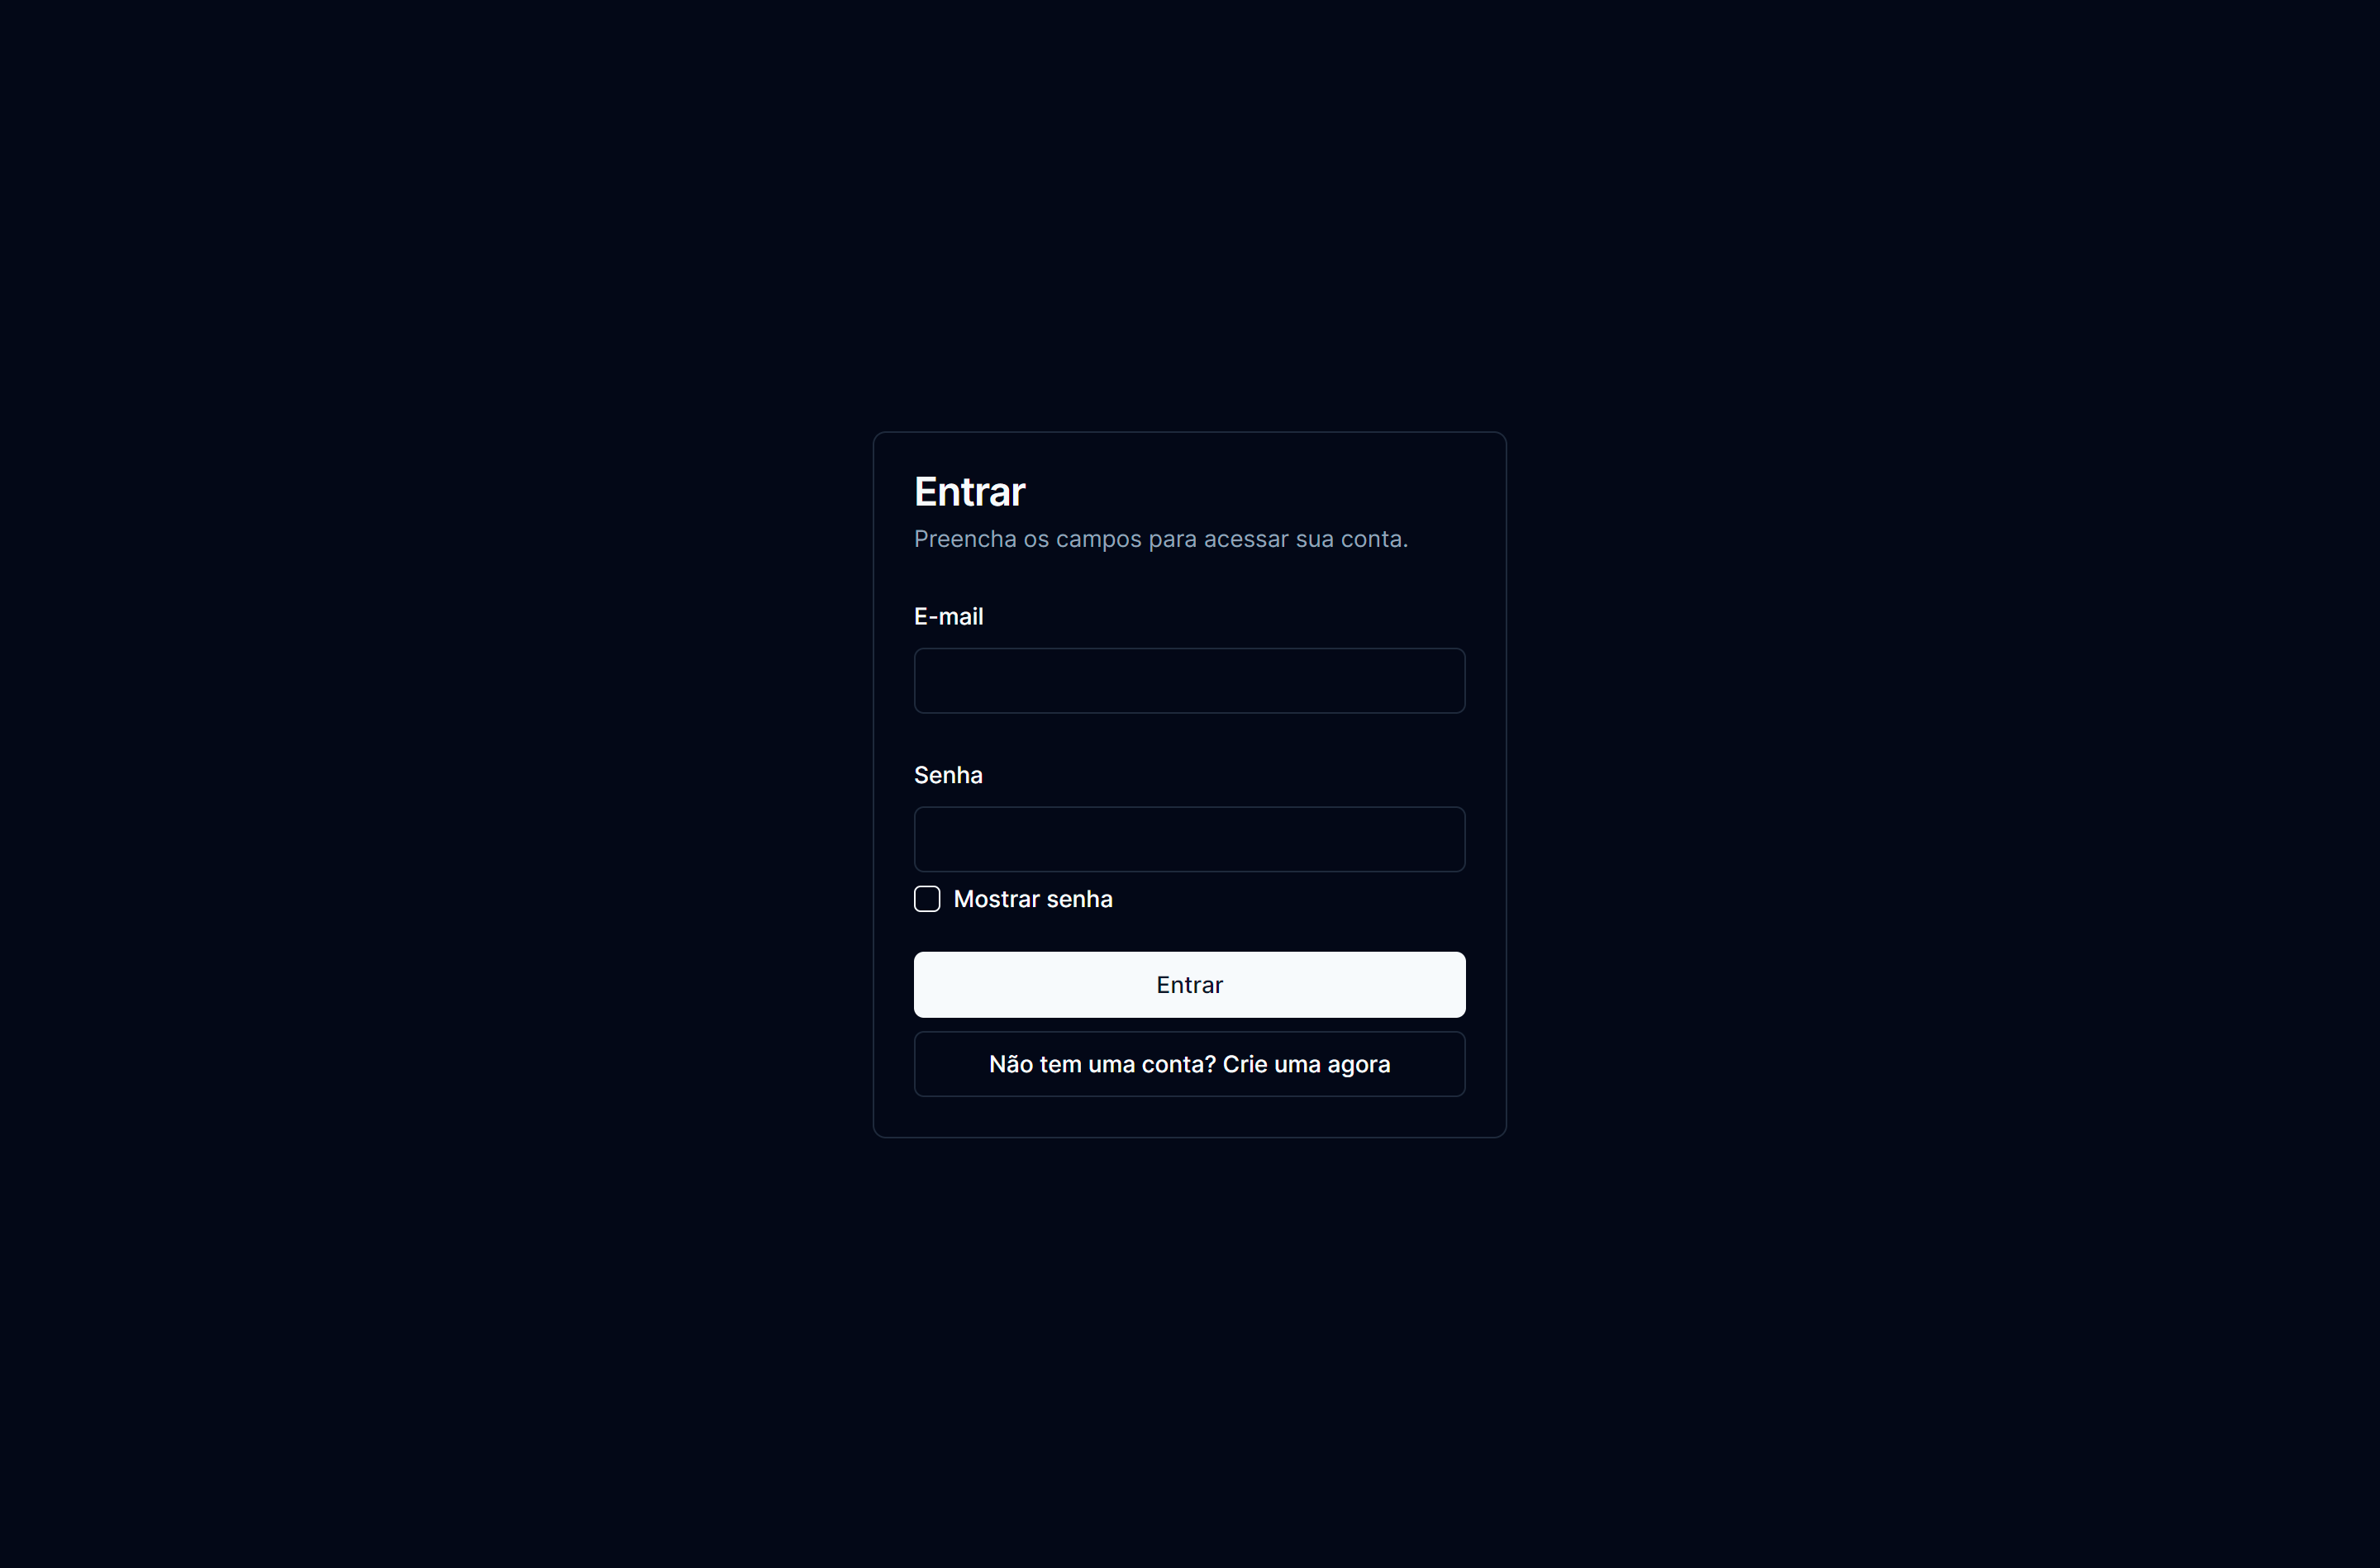
\includegraphics[width=0.8\textwidth]{assets/codeboard/login-page.png}
    \caption{Página de login da plataforma Codeboard UERJ.}
    \label{fig:login-page}
\end{figure}

No caso do usuário não possuir uma conta, ele pode clicar no link de cadastro e preencher o formulário de cadastro. Após o cadastro, o  usuário também é redirecionado para a tela inicial.

\begin{figure}[H]
    \centering
    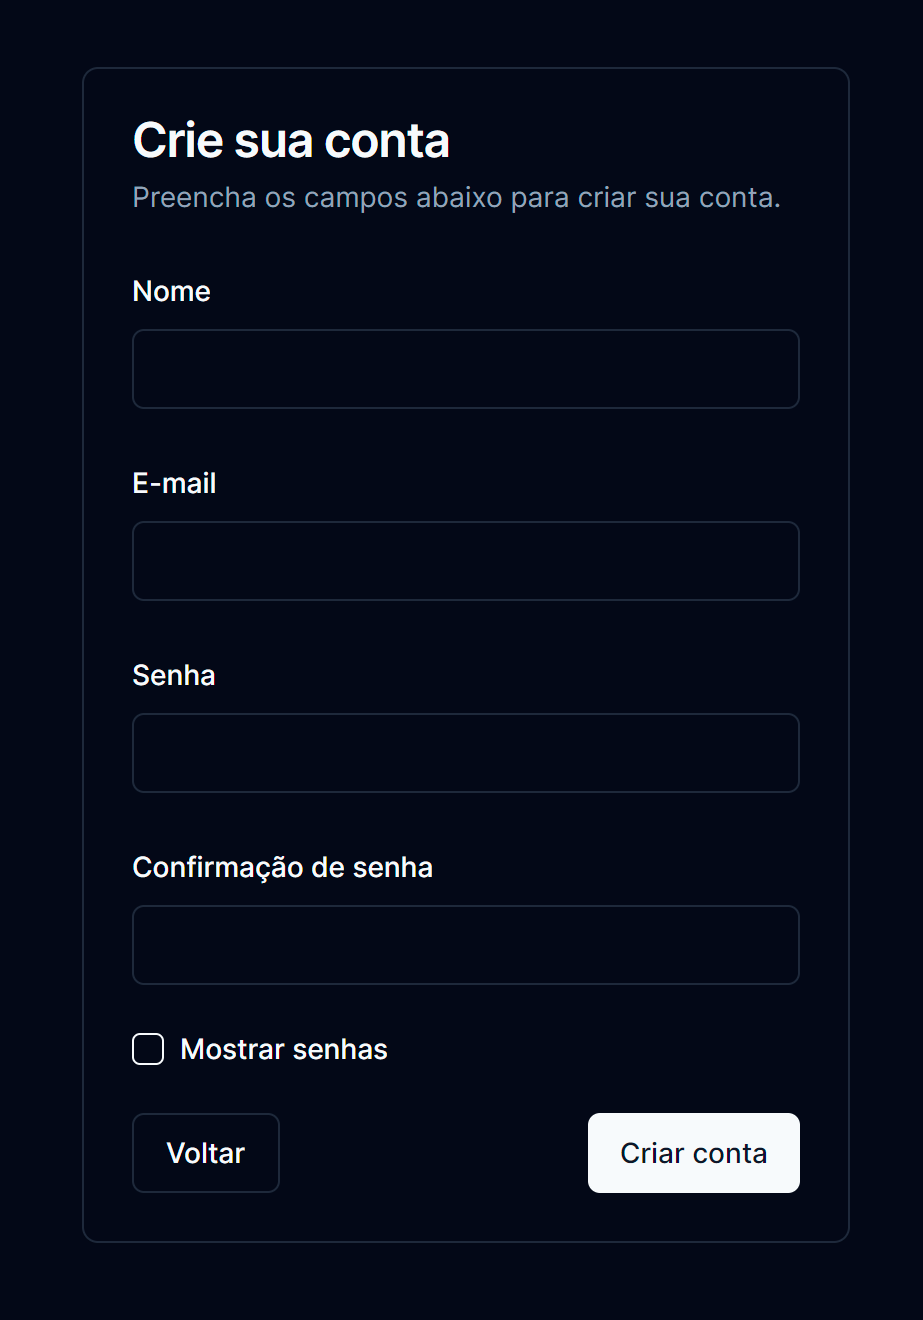
\includegraphics[width=0.8\textwidth]{assets/codeboard/signup-page.png}
    \caption{Página de cadastro da plataforma Codeboard UERJ.}
    \label{fig:signup-page}
\end{figure}

Durante o processo de autenticação, a plataforma utiliza tokens de autenticação para manter o usuário autenticado. O token é gerado no servidor e enviado para o cliente, onde é armazenado no navegador por meio de cookies. O token é utilizado para autenticar o usuário em todas as requisições feitas para o servidor, garantindo que o usuário esteja autenticado em todas as páginas da plataforma.

\subsubsection{Gerenciamento de Salas}

A funcionalidade de gerenciamento de salas permite que o professor crie, edite e acesse salas de aula. A criação de uma sala é feita através de um formulário que solicita o nome da sala e a descrição da atividade prática. Após a criação, o professor pode acessar a sala e adicionar alunos a ela.

\begin{figure}[H]
    \centering
    \includegraphics[width=0.8\textwidth]{diagrams/user-room-flow.png}
    \caption{Diagrama do fluxo de gerenciamento de salas.}
    \label{fig:user-room-flow}
\end{figure}

A tela de listagem de salas é a primeira tela exibida ao usuário após o login. Ela exibe todas as salas em que o usuário é dono ou membro. O usuário pode acessar uma sala clicando no botão de acesso, que o redireciona para a tela da sala.

\begin{figure}[H]
    \centering
    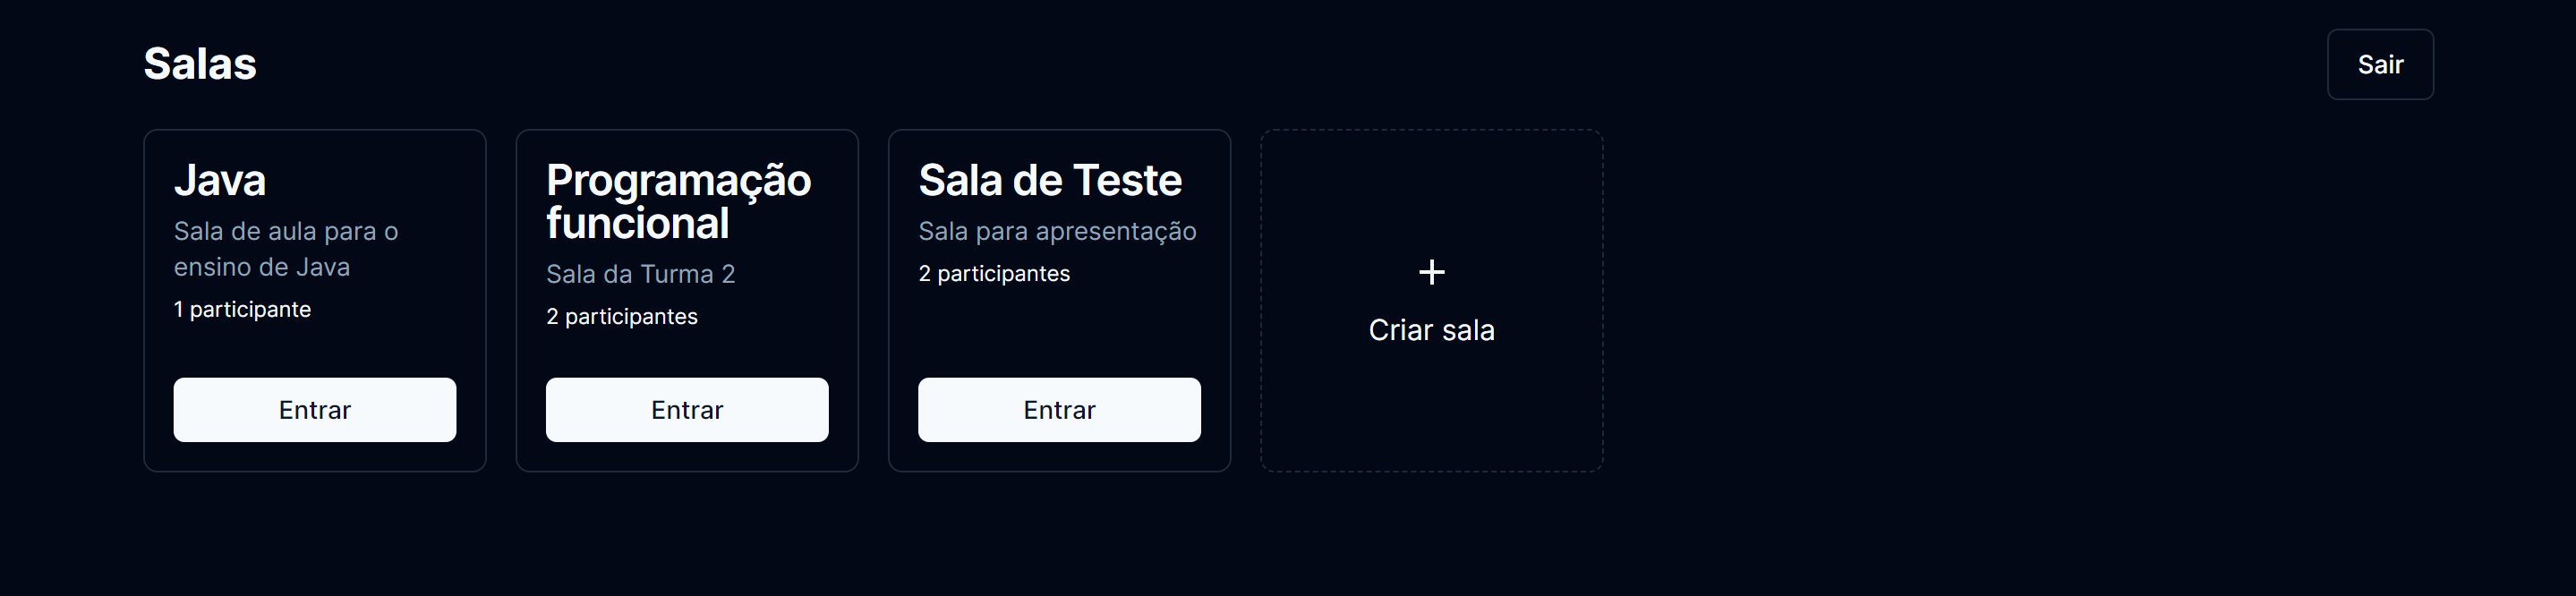
\includegraphics[width=0.8\textwidth]{assets/codeboard/rooms-page.png}
    \caption{Página de listagem de salas da plataforma Codeboard UERJ.}
    \label{fig:rooms-page}
\end{figure}

Nesta mesma tela da figura \ref{fig:rooms-page}, o usuário pode criar uma nova sala clicando no botão de criação de sala. O usuário é redirecionado para uma tela de criação de sala, onde ele pode preencher o nome e a descrição da sala. Após a criação, o usuário é redirecionado para a tela da sala.

\begin{figure}[H]
    \centering
    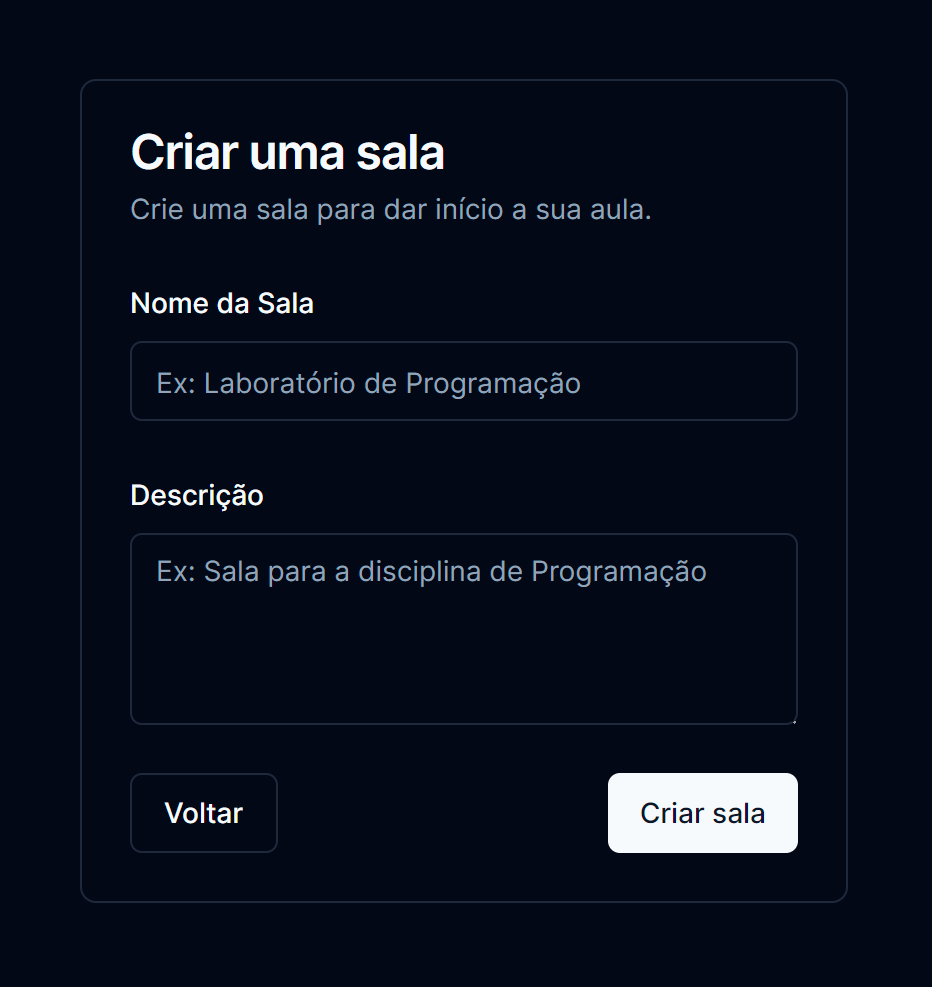
\includegraphics[width=0.8\textwidth]{assets/codeboard/create-room-page.png}
    \caption{Página de criação de sala da plataforma Codeboard UERJ.}
    \label{fig:create-room-page}
\end{figure}

Para adicionar alunos à sala, o usuário pode clicar num botão de adição de participantes representado por um ícone de usuário. A plataforma exibe um modal com um campo de e-mail, onde o usuário pode informar o e-mail do aluno que deseja adicionar à sala. Após a adição, o aluno se torna membro da sala e pode acessá-la.

\begin{figure}[H]
    \centering
    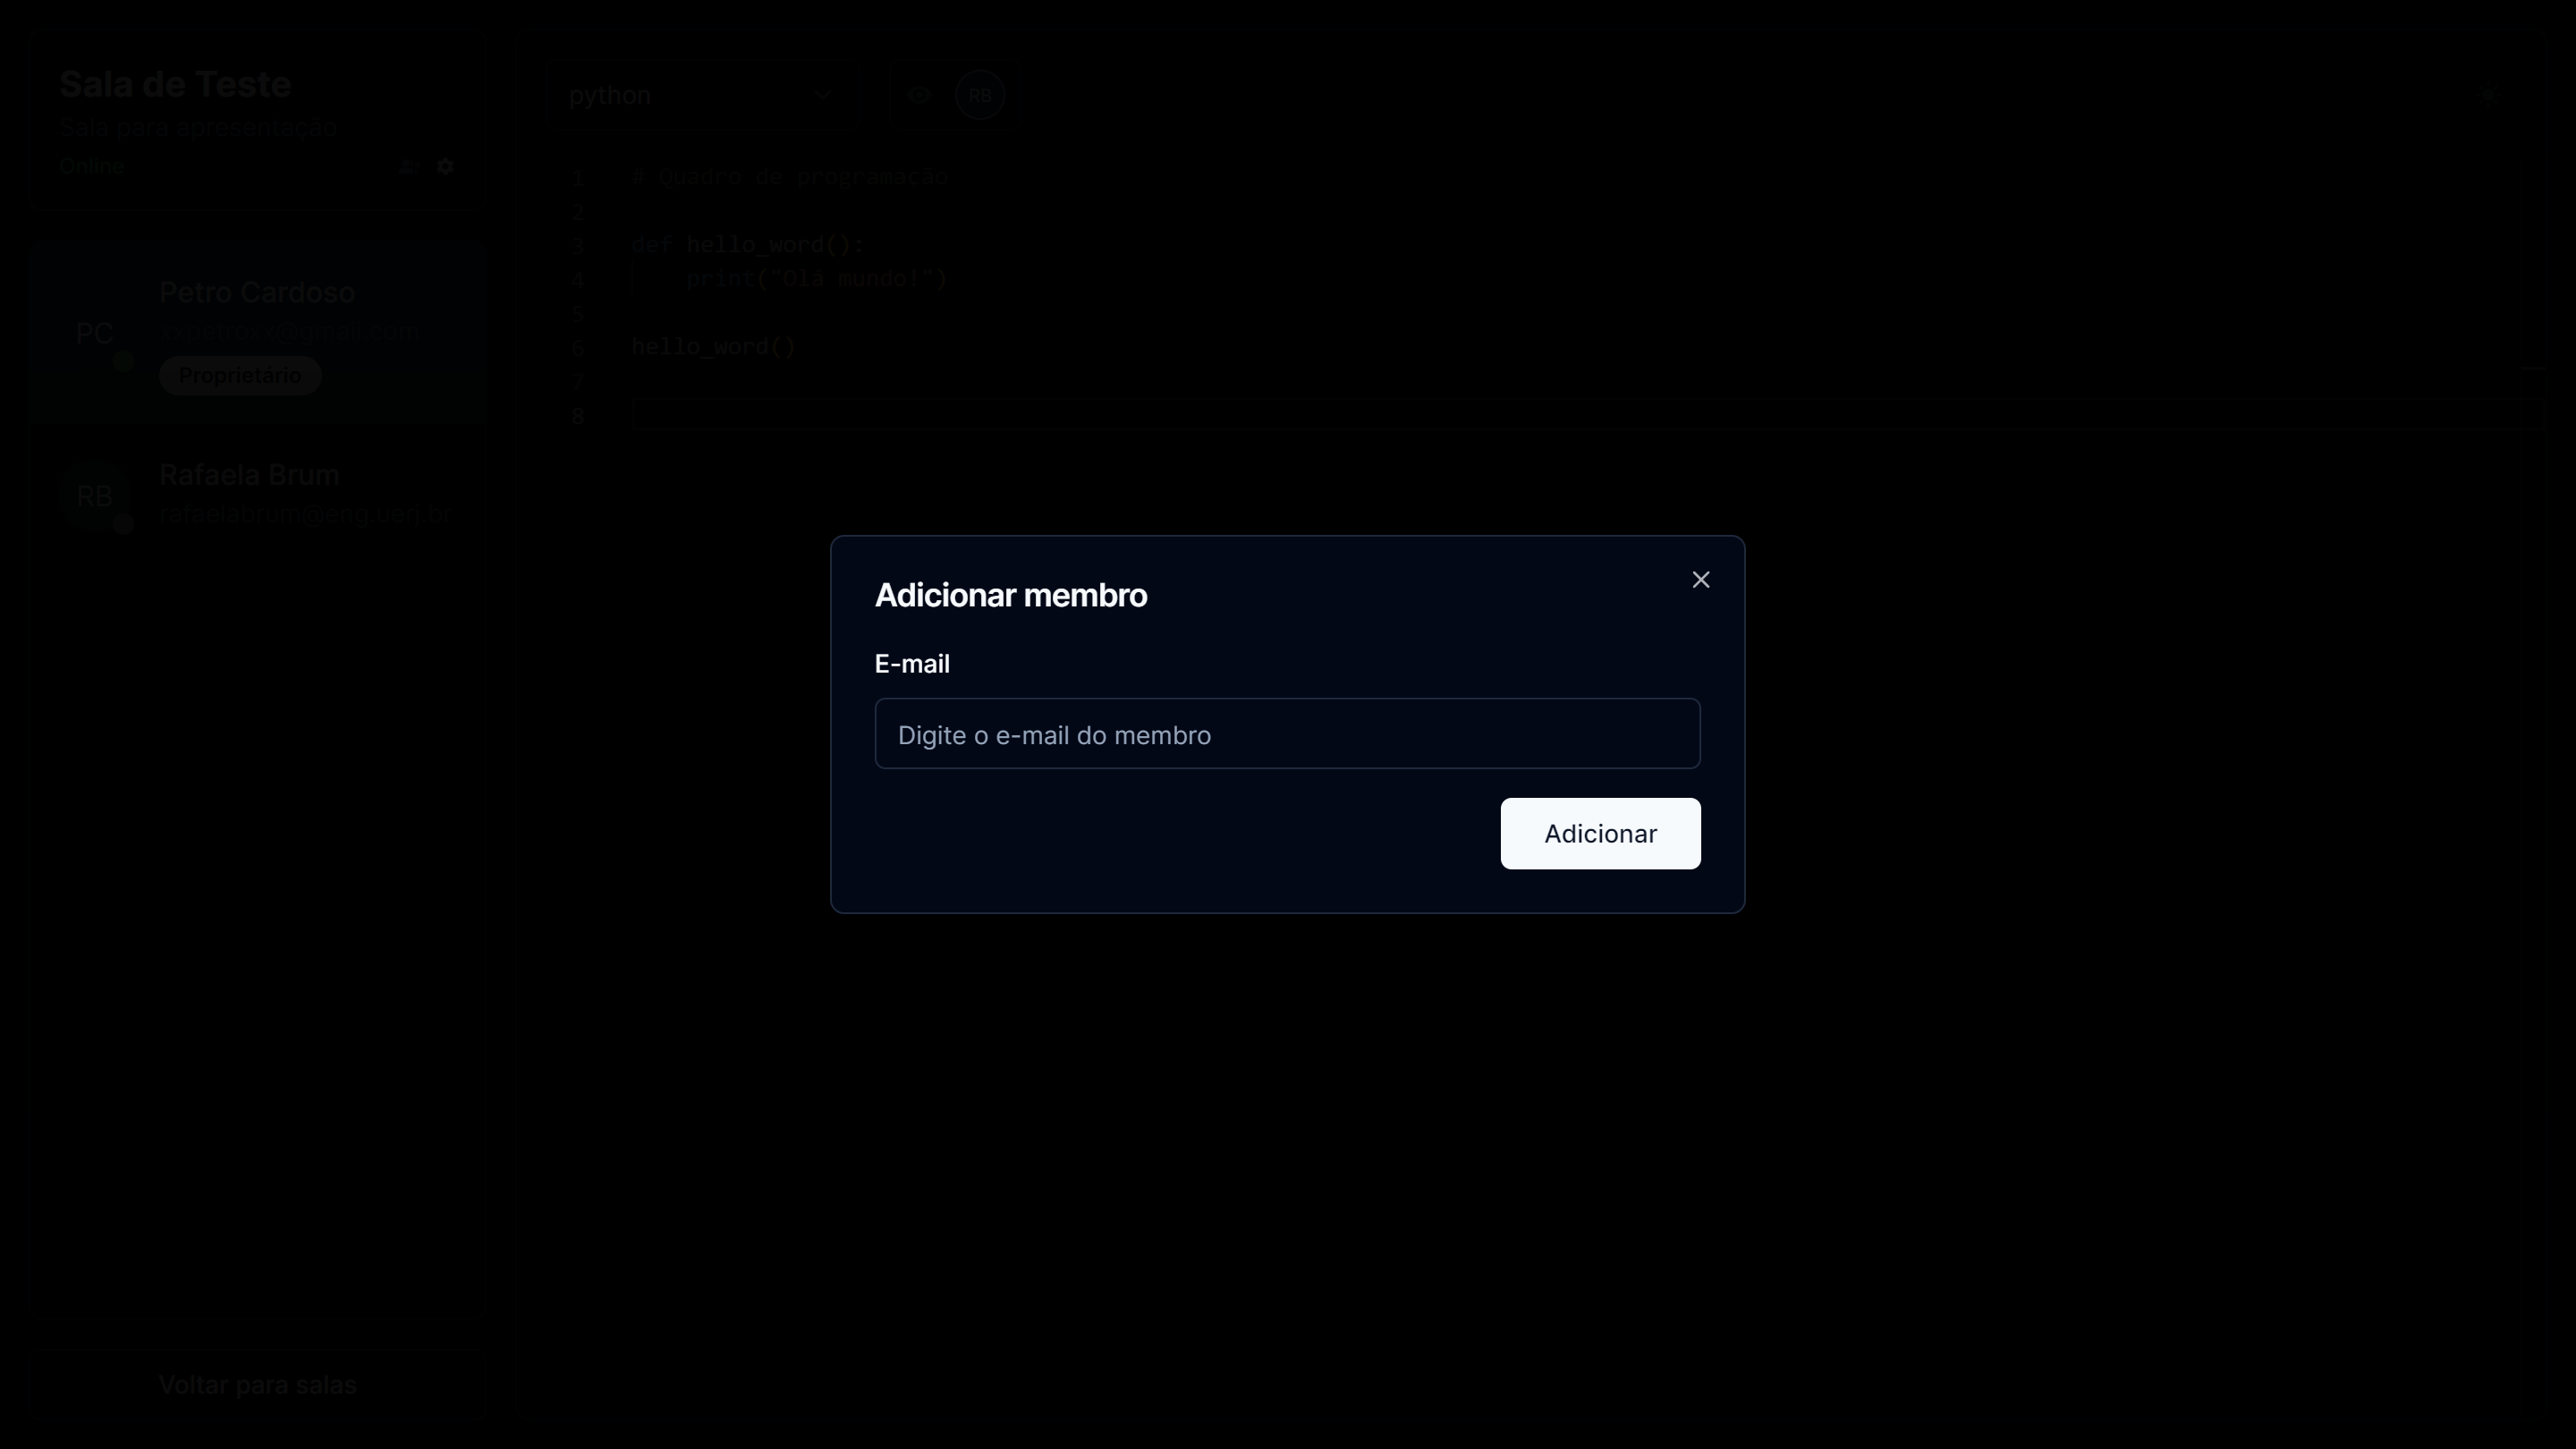
\includegraphics[width=0.8\textwidth]{assets/codeboard/add-member-modal.png}
    \caption{Página de adição de alunos à sala da plataforma Codeboard UERJ.}
    \label{fig:add-member-modal}
\end{figure}

\subsubsection{Quadro de Programação em Tempo Real}

A funcionalidade de quadro de programação em tempo real é a principal funcionalidade da plataforma. Ela permite que os alunos escrevam códigos de programação diretamente no navegador, sem a necessidade de instalar um ambiente de desenvolvimento integrado (IDE).

Para acessar o quadro de programação, o usuário deve acessar a sala desejada. A plataforma exibe uma tela dividida em dois módulos, o módulo lateral de seleção de usuário e o módulo central de edição de código.

\begin{figure}[H]
    \centering
    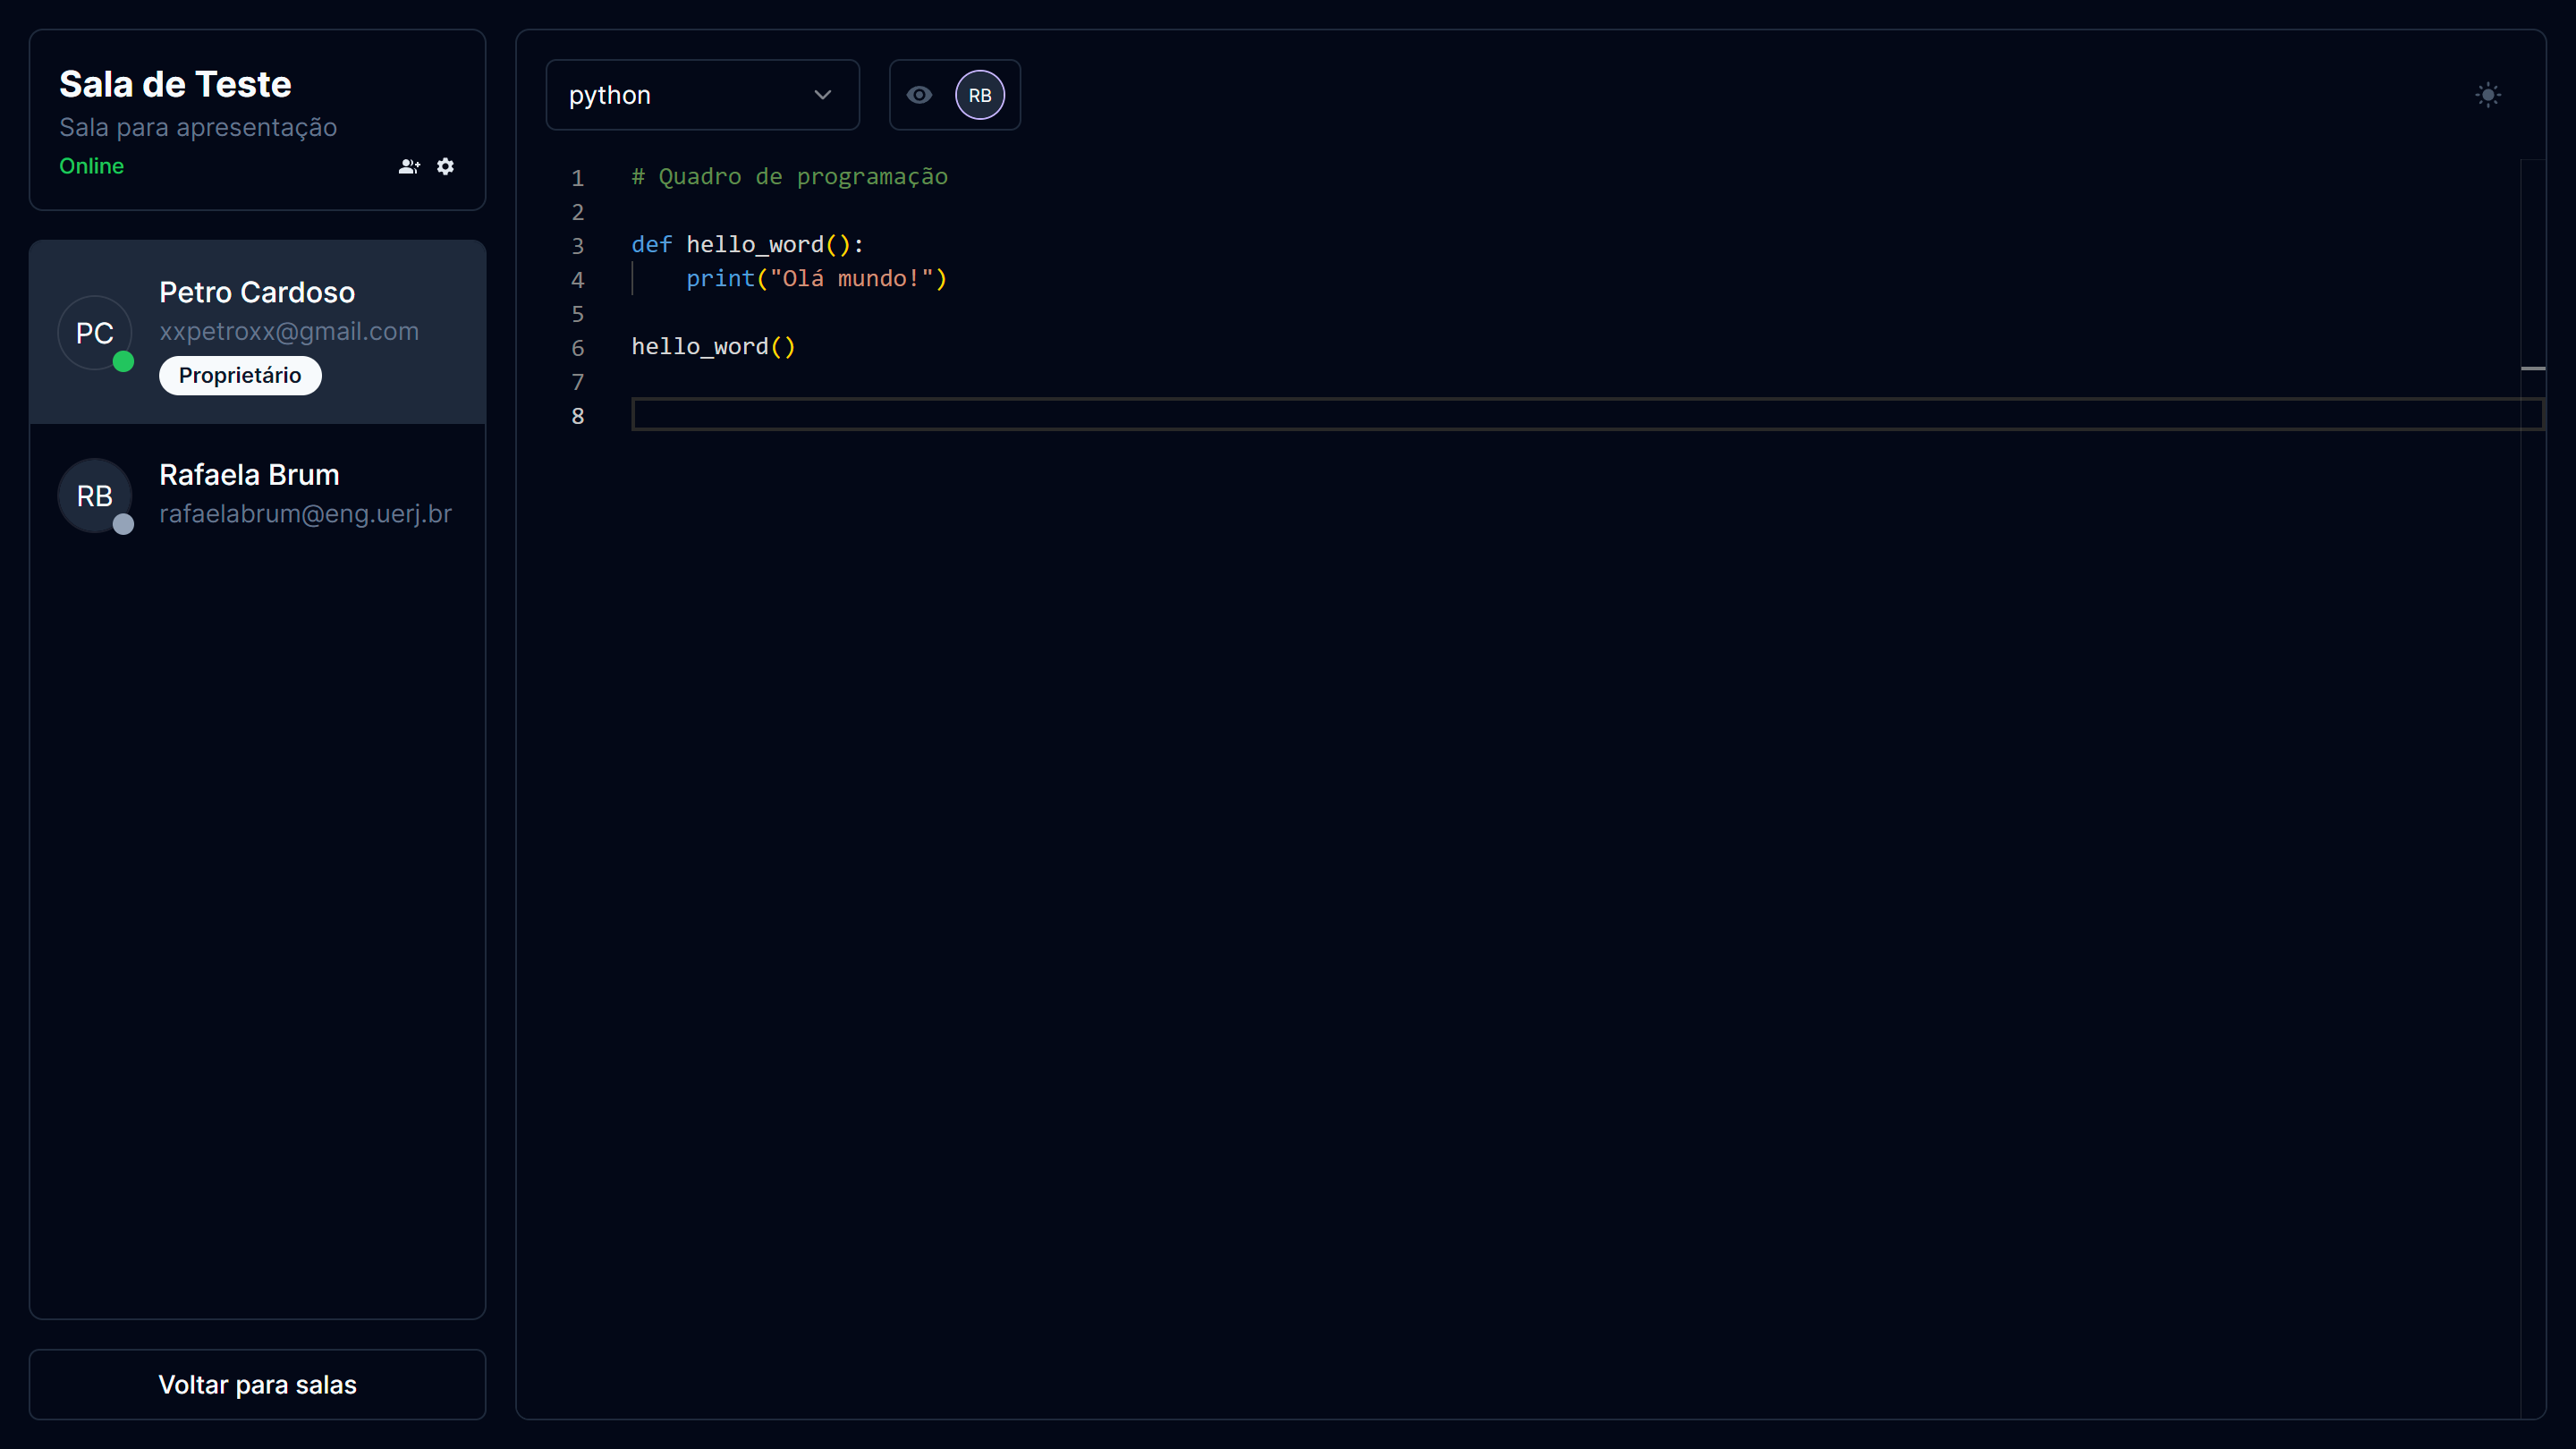
\includegraphics[width=0.8\textwidth]{assets/codeboard/room-details-page.png}
    \caption{Página da sala de programação da plataforma Codeboard UERJ.}
    \label{fig:room-details-page}
\end{figure}


Como mostra a figura \ref{fig:room-details-page}, o módulo lateral exibe a lista de participantes da sala. Para cada membro listado, é exibido o nome, a foto de perfil e indicadores para caso ele esteja online ou esteja editando o seu próprio código. O usuário pode selecionar outro membro da sala na lista lateral para visualizar e interagir com o código dele.

Caso o usuário já esteja com si mesmo selecionado, ele poderá editar o próprio código, trocar de linguagem de programação e visualizar quem está visualizando seu código. O código é salvo automaticamente a cada edição realizada pelo usuário.

Acima do módulo lateral, a plataforma exibe o nome da sala e sua descrição. Caso o usuário seja o dono da sala, também serão exibidos os botões de adição de participantes e de configuração da sala. O botão de adição de participantes permite que o usuário adicione novos participantes à sala, enquanto o botão de configuração permite que o usuário edite o nome e a descrição da sala.

\begin{figure}[H]
    \centering
    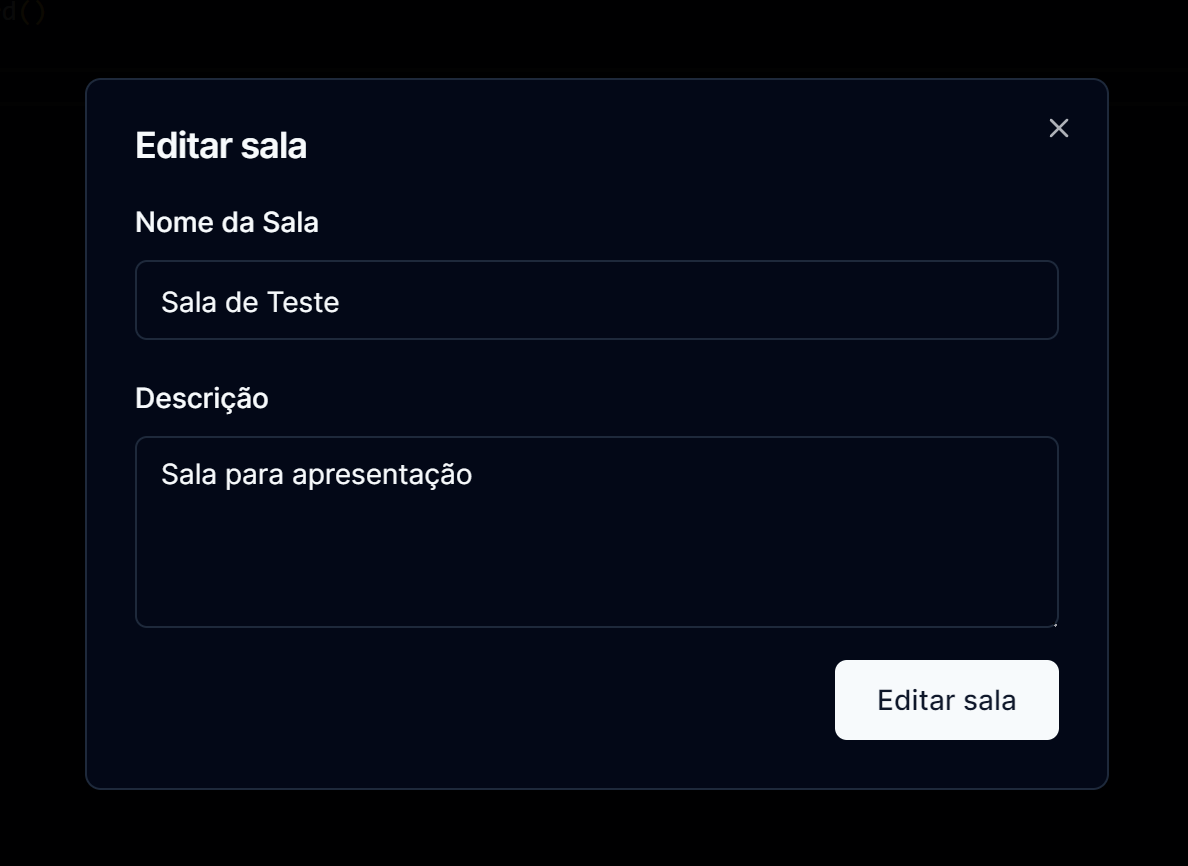
\includegraphics[width=0.8\textwidth]{assets/codeboard/edit-room-modal.png}
    \caption{Modal de configuração de sala da plataforma Codeboard UERJ.}
    \label{fig:edit-room-modal}
\end{figure}


Abaixo do módulo lateral, a plataforma exibe um botão de saída da sala. Ao clicar neste botão, o usuário é redirecionado para a tela de listagem de salas, onde ele pode acessar outras salas ou criar uma nova sala.

O módulo central exibe o editor de código. Este editor suporta as funcionalidades básicas de um IDE, como coloração de sintaxe, auto-completar e formatação de código. Durante a visualização do código de outro usuário, o usuário pode somente fazer marcações que são exibidas em tempo real para o outros usuários presentes no quadro.

\begin{figure}[H]
    \centering
    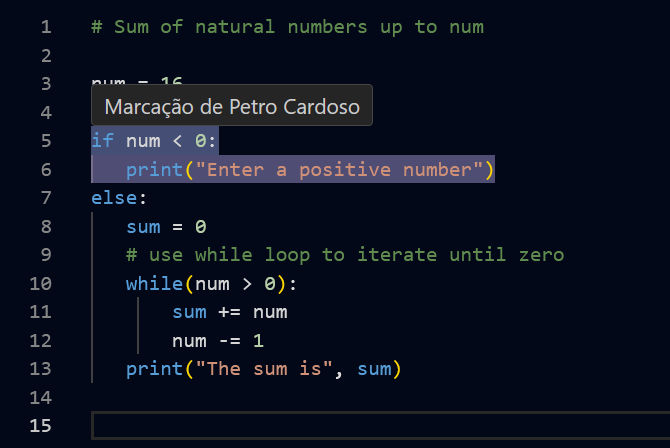
\includegraphics[width=0.8\textwidth]{assets/codeboard/code-editor-user-highlight.png}
    \caption{Marcação de código na plataforma Codeboard UERJ.}
    \label{fig:code-editor-user-highlight}
\end{figure}

Na parte superior do editor, o usuário pode selecionar a linguagem de programação desejada. A plataforma suporta as linguagens de programação mais utilizadas, como C, C++, Java, Python, JavaScript, entre outras. A seleção da linguagem de programação altera a coloração de sintaxe do editor, facilitando a escrita e a leitura do código.

\begin{figure}[H]
    \centering
    
\includegraphics[width=0.8\textwidth]{assets/codeboard/code-editor-toolbar.png}
    \caption{Barra de ferramentas do editor de código da plataforma Codeboard UERJ.}
    \label{fig:code-editor-toolbar}
\end{figure}

Ao lado da seleção de linguagem, o usuário pode visualizar quem está visualizando o seu código no momento. A plataforma exibe uma lista horizontal com estes visualizadores, permitindo que ele saiba quem está acompanhando o seu progresso.


\subsubsection{Regras de Negócio}

Existem algumas regras de negócio que devem ser seguidas para garantir o bom funcionamento da plataforma. Estas regras são implementadas no backend da plataforma e são responsáveis por validar os dados dos usuários e das salas, bem como garantir a segurança e a integridade dos dados.

\paragraph{Autenticação}

\begin{itemize}
    \item \textbf{Cadastro de Usuários}: A plataforma deve fornecer um mecanismo de cadastro de usuários que permita aos usuários se registrarem na plataforma. Para isso, é necessário solicitar os dados dos usuários, como nome, e-mail e senha, e armazená-los de forma segura e protegida no banco de dados.
    \item \textbf{Validação de Dados}: A plataforma deve garantir que os dados dos usuários sejam válidos e consistentes. Para isso, é necessário validar os dados dos usuários durante o processo de cadastro e login e garantir que os dados sejam consistentes e íntegros.
    \item \textbf{Proteção de Dados}: A plataforma deve garantir que os dados dos usuários sejam protegidos e seguros. Para isso, é necessário armazenar os dados dos usuários de forma segura e protegida, utilizando técnicas de criptografia e hash de senhas.
    \item \textbf{Login de Usuários}: A plataforma deve garantir que somente usuários cadastrados possam fazer login. Para isso, é necessário verificar se o e-mail e a senha informados são válidos durante o processo de login e gerar um token de autenticação para manter o usuário autenticado.
    \item \textbf{Gerenciamento de Sessões}: A plataforma deve garantir que as sessões dos usuários sejam gerenciadas de forma segura e eficiente. Para isso, é necessário gerar tokens de autenticação para manter os usuários autenticados e garantir que as sessões sejam encerradas após um período de inatividade.
    \item \textbf{Restrição de Acesso}: A plataforma deve garantir que somente usuários autenticados tenham acesso às funcionalidades da plataforma. Para isso, é necessário verificar se o usuário está autenticado antes de permitir o acesso às funcionalidades.
\end{itemize}

\paragraph{Gerenciamento de Salas}

\begin{itemize}
    \item \textbf{Criação de Salas}: A plataforma deve fornecer um mecanismo de criação de salas que permita aos usuários criarem novas salas. Para isso, é necessário solicitar os dados das salas, como nome e descrição, e armazená-los de forma segura e protegida no banco de dados.
    \item \textbf{Validação de Dados}: A plataforma deve garantir que os dados das salas sejam válidos e consistentes. Para isso, é necessário validar os dados das salas durante o processo de criação e edição e garantir que os dados sejam consistentes e íntegros.
    \item \textbf{Restrição de Acesso}: A plataforma deve garantir que somente participantes da sala tenham acesso à ela. Para isso, é necessário verificar se o usuário é dono ou membro da sala antes de permitir o acesso à sala.
    \item \textbf{Gerenciamento de Participantes}: A plataforma deve fornecer um mecanismo de adição e remoção de participantes que permita aos usuários gerenciarem os participantes das salas. Para isso, é necessário verificar se o usuário é dono da sala antes de permitir a adição ou remoção de participantes.
    \item \textbf{Restrição de Edição}: A plataforma deve garantir que somente o dono da sala possa editar os dados da sala. Para isso, é necessário verificar se o usuário é dono da sala antes de permitir a edição dos dados da sala.
\end{itemize}

\paragraph{Quadro de Programação}

\begin{itemize}
    \item \textbf{Editor em Tempo Real}: A plataforma deve fornecer um mecanismo de edição de código em tempo real que permita aos usuários escrever códigos de programação diretamente no navegador. Para isso, é necessário implementar um editor de código que suporte as funcionalidades básicas de um IDE, como coloração de sintaxe, auto-completar e formatação de código.
    \item \textbf{Restrição de Escrita}: A plataforma deve garantir que não haja conflitos de escrita durante a edição do código em tempo real. Para isso, é necessário implementar um mecanismo de bloqueio de escrita que permita que somente o proprietário do código possa editá-lo.
    \item \textbf{Marcação de Código}: A plataforma deve fornecer um mecanismo de marcação de texto que permita aos usuários visualizarem e interagirem com o código de outros usuários. Para isso, é necessário implementar um mecanismo de marcação que exiba as alterações em tempo real para os outros usuários presentes no quadro.
    \item \textbf{Seleção de Linguagem}: A plataforma deve fornecer um mecanismo de seleção de linguagem que permita aos usuários escolher a linguagem de programação desejada. Para isso, é necessário implementar um seletor de linguagem que altere a coloração de sintaxe do editor de código.
    \item \textbf{Visualização de Usuários}: A plataforma deve fornecer um mecanismo de visualização de usuários que permita aos usuários saber quem está visualizando o seu código. Para isso, é necessário implementar uma lista de visualizadores que exiba os usuários presentes no quadro.
\end{itemize}

\paragraph{Lista de Participantes}

\begin{itemize}
    \item \textbf{Visualização de Participantes}: A plataforma deve fornecer um mecanismo de visualização de participantes que permita aos usuários saber quem está presente na sala. Para isso, é necessário implementar uma lista de participantes que exiba os usuários presentes na sala.
    \item \textbf{Indicadores de Presença}: A plataforma deve fornecer um mecanismo de indicação de presença que permita aos usuários saber quem está online e quem está editando o código. Para isso, é necessário implementar indicadores de presença que exibam se o usuário está online e se está editando o código.
    \item \textbf{Seleção de Participantes}: A plataforma deve fornecer um mecanismo de seleção de participantes que permita aos usuários visualizarem e interagirem com o código de outros participantes. Para isso, é necessário implementar um seletor de participantes que permita selecionar o participante desejado.
\end{itemize}


\subsection{Arquitetura da Plataforma}
% Revisado

Nesta seção, será apresentada a arquitetura da plataforma Codeboard UERJ. A plataforma é estruturada em três camadas principais: o backend, o banco de dados e o frontend. Cada uma dessas camadas desempenha um papel específico na plataforma, sendo responsável pelas regras de negócio, o armazenamento de dados e a interface com o usuário, respectivamente.

\subsubsection{Backend}
% Revisado

O backend da plataforma é responsável pela implementação das regras de negócio da aplicação. Ele é composto por um servidor NodeJS que utiliza dois métodos de comunicação: REST API e WebSockets. A REST API é usada para comunicação assíncrona entre o cliente e o servidor, enquanto os WebSockets são utilizados para permitir a comunicação em tempo real entre os usuários.

\begin{figure}[H]
    \centering
    \includegraphics[width=0.75\textwidth]{diagrams/backend-architecture.png}
    \caption{Arquitetura do backend da plataforma Codeboard UERJ.}
    \label{fig:backend-architecture}
\end{figure}

Conforme a arquitetura do backend ilustrada na Figura \ref{fig:backend-architecture}, a comunicação entre o cliente e o servidor ocorre através de duas interfaces principais: REST API e WebSockets. A REST API fornece um conjunto de rotas que permitem ao cliente acessar funcionalidades da plataforma, como autenticação de usuários, gerenciamento de salas e edição de código. Os WebSockets, por sua vez, são utilizados para viabilizar a comunicação em tempo real entre os usuários, possibilitando a edição colaborativa de código.


\subsubsection{Banco de Dados NoSQL}
% Revisado

A plataforma utiliza o MongoDB como banco de dados, um sistema NoSQL orientado a documentos. O MongoDB foi escolhido por sua flexibilidade, capacidade de escalabilidade horizontal e eficiência no armazenamento de grandes volumes de dados. Além disso, sua integração simples com o NodeJS o torna uma escolha natural para a plataforma Codeboard UERJ.

O banco de dados é organizado em duas coleções principais: a coleção de usuários e a coleção de salas. A coleção de usuários armazena informações dos usuários cadastrados na plataforma, como nome, e-mail e senha. Já a coleção de salas guarda os dados das salas criadas pelos usuários, incluindo nome, descrição e participantes.

\begin{figure}[H]
    \centering
    \includegraphics[width=0.7\textwidth]{diagrams/database-schema.png}
    \caption{Esquema do banco de dados da plataforma Codeboard UERJ.}
    \label{fig:database-schema}
\end{figure}

Conforme o esquema do banco de dados ilustrado na Figura \ref{fig:database-schema}, a coleção "User", responsável por armazenar os dados dos usuários, inclui os seguintes campos:

\begin{table}[H]
    \centering
    \renewcommand{\arraystretch}{1.3} 
    \begin{tabular}{|c|c|c|c|}
        \hline
        \textbf{Campo} & \textbf{Descrição}             & \textbf{Tipo} & \textbf{Obrigatório} \\
        \hline
        \_id           & Identificador único do usuário & ObjectId      & Sim                  \\
        \hline
        name           & Nome do usuário                & String        & Sim                  \\
        \hline
        email          & E-mail do usuário              & String        & Sim                  \\
        \hline
        password       & Hash da senha do usuário       & String        & Sim                  \\
        \hline
        createdAt      & Data de criação do usuário     & Date          & Sim                  \\
        \hline
    \end{tabular}
    \caption{Campos da coleção "User" do banco de dados da plataforma Codeboard UERJ.}
    \label{tab:user-collection-fields}
\end{table}

É importante destacar que a coleção de usuários possui um campo "password" que armazena o hash da senha do usuário. Essa prática é adotada por motivos de segurança, garantindo que a senha do usuário não seja armazenada em texto puro no banco de dados, o que poderia expor as informações dos usuários em caso de vazamento de dados.

A coleção "Room", responsável por armazenar os dados das salas, contém os seguintes campos:

\begin{table}[H]
    \centering
    \renewcommand{\arraystretch}{1.3} 
    \begin{tabular}{|c|c|c|c|}
        \hline
        \textbf{Campo} & \textbf{Descrição}             & \textbf{Tipo}   & \textbf{Obrigatório} \\
        \hline
        \_id           & Identificador único da sala    & ObjectId        & Sim                  \\
        \hline
        name           & Nome da sala                   & String          & Sim                  \\
        \hline
        description    & Descrição da sala              & String          & Não                  \\
        \hline
        owner          & Identificador do dono da sala  & ObjectId        & Sim                  \\
        \hline
        members        & Lista de participantes da sala & Array<ObjectId> & Não                  \\
        \hline
        createdAt      & Data de criação da sala        & Date            & Sim                  \\
        \hline
    \end{tabular}
    \caption{Campos da coleção "Room" do banco de dados da plataforma Codeboard UERJ.}
    \label{tab:room-collection-fields}
\end{table}


Podemos observar que a coleção de salas possui os campos "owner" e "members" que armazenam os identificadores do dono e dos participantes da sala, respectivamente. Estes campos são utilizados para estabelecer a relação entre os usuários e as salas.

A coleção "Board", responsável por armazenar os dados dos quadros de programação, contém os seguintes campos:

\begin{table}[H]
    \centering
    \renewcommand{\arraystretch}{1.3} 
    \begin{tabular}{|c|c|c|c|}
        \hline
        \textbf{Campo} & \textbf{Descrição}             & \textbf{Tipo} & \textbf{Obrigatório} \\
        \hline
        \_id           & Identificador único do quadro  & ObjectId      & Sim                  \\
        \hline
        user         & Identificador do usuário dono do quadro & ObjectId      & Sim                  \\
        \hline
        room         & Identificador da sala do quadro & ObjectId      & Sim                  \\
        \hline
        language       & Linguagem de programação       & String        & Sim                  \\
        \hline
        content           & Código de programação          & String        & Sim                  \\
        \hline
        updatedAt      & Data da última atualização      & Date          & Não                  \\
        \hline
        createdAt      & Data de criação      & Date          & Sim                  \\
        \hline
    \end{tabular}
    \caption{Campos da coleção "Board" do banco de dados da plataforma Codeboard UERJ.}
    \label{tab:board-collection-fields}
\end{table}

A coleção de "Board" possui os campos "user" e "room" que armazenam os identificadores do usuário dono do quadro e da sala do quadro, respectivamente. Esses campos são utilizados para estabelecer a relação entre os usuários, as salas e os quadros de programação.


Embora o banco de dados seja NoSQL, a plataforma Codeboard UERJ adota um esquema de dados bem definido para assegurar a consistência e a integridade das informações. Esse esquema é estabelecido no backend da plataforma com o auxílio do pacote "mongoose", que simplifica a modelagem dos dados e a interação com o banco de dados MongoDB.

\subsubsection{Comunicação Síncrona via REST API}
% Revisado

A REST API é formada por um conjunto de rotas que possibilitam ao cliente acessar as funcionalidades da plataforma. Essas rotas são implementadas com o framework ExpressJS, que facilita a criação de rotas e middlewares em aplicações NodeJS.

Na REST API, existem três tipos principais de rotas: de autenticação, de usuários e de salas. As rotas de autenticação são responsáveis pela criação e autenticação de usuários, enquanto as rotas de usuários permitem o acesso e a atualização dos dados dos usuários. Já as rotas de salas são utilizadas para criar, acessar e gerenciar as salas.

\begin{table}[H]
    \centering
    \renewcommand{\arraystretch}{1.3} 
    \begin{tabular}{|c|c|c|c|}
        \hline
        \textbf{Método} & \textbf{Rota}                  & \textbf{Descrição}            & \textbf{Autenticação} \\
        \hline
        GET             & /api/health                    & Verifica o status do servidor & Não                   \\
        \hline
        POST            & /api/auth/signup               & Cadastra um novo usuário      & Não                   \\
        POST            & /api/auth/login                & Autentica um usuário          & Não                   \\
        \hline
        GET             & /api/user                      & Retorna os dados do usuário   & Sim                   \\
        PUT             & /api/user                      & Edita os dados do usuário     & Sim                   \\
        \hline
        GET             & /api/rooms                     & Lista todas as salas          & Sim                   \\
        POST            & /api/rooms                     & Cria uma nova sala            & Sim                   \\
        GET             & /api/rooms/:id                 & Retorna uma sala específica   & Sim                   \\
        PUT             & /api/rooms/:id                 & Edita uma sala específica     & Sim                   \\
        POST            & /api/rooms/:id/members         & Adiciona um membro à sala     & Sim                   \\
        DELETE          & /api/rooms/:id/members/:userId & Remove um membro da sala      & Sim                   \\
        \hline
    \end{tabular}
    \caption{Rotas da REST API da plataforma Codeboard UERJ.}
    \label{tab:rest-api-routes}
\end{table}


\subsubsection{Sistema de Autenticação}
% Revisado

As rotas descritas na tabela \ref{tab:rest-api-routes} que requerem autenticação, são protegidas por um middleware que verifica se o usuário está autenticado antes de permitir o acesso. A autenticação do usuário na plataforma é realizada através de um token, que é gerado no servidor e enviado ao cliente após o login. 

O token de autenticação é gerado utilizando o pacote "jsonwebtoken", que implementa o padrão JWT (JSON Web Token). A escolha do JWT como mecanismo de autenticação foi motivada pela necessidade de suportar a infraestrutura horizontal da plataforma, que facilita a escalabilidade e a distribuição dos servidores. Como o JWT é um mecanismo stateless, não é necessário armazenar o estado da sessão no servidor. Isso o torna ideal para aplicações distribuídas e escaláveis, pois o estado da sessão é armazenado no próprio token, que é enviado ao cliente.

O token é criado com base no ID do usuário e uma chave secreta, que é mantida nos servidores. Esse token é assinado com a chave secreta e enviado ao cliente, onde é armazenado no navegador por meio de cookies. A cada requisição feita ao servidor, o token é utilizado para autenticar o usuário, garantindo sua autenticidade em todas as páginas da plataforma.

O token de autenticação tem um tempo de expiração configurado no servidor. Após esse período, o token é invalidado, e o usuário é automaticamente desconectado da plataforma.

\subsubsection{Banco de Dados Chave-Valor}
% Revisado OK

A plataforma Codeboard UERJ utiliza o Redis, um banco de dados chave-valor em memória, para armazenar dados temporários relacionados à interação em tempo real, como a lista de usuários online, o código ativo nos quadros de programação e a lista de visualizadores dos quadros. O Redis foi escolhido devido à sua eficiência no processamento de grandes volumes de dados em memória, oferecendo alto desempenho, baixa latência e suporte robusto à escalabilidade horizontal.

A adoção do Redis é comum em sistemas que demandam alta disponibilidade e tempos de resposta rápidos, características fundamentais para a experiência de colaboração simultânea proporcionada pela Codeboard UERJ. O Redis não apenas facilita a manipulação de dados em tempo real, mas também garante que os dados temporários sejam gerenciados de maneira eficiente, minimizando o uso excessivo de recursos.

A Tabela \ref{tab:key-value-database} descreve a estrutura do banco de dados chave-valor utilizado na plataforma, evidenciando como os dados são organizados em namespaces. Cada namespace reflete um contexto específico da aplicação, como as salas de colaboração ou os quadros de programação, e cada um possui um tempo de expiração associado, normalmente configurado para 1 dia. Essa expiração automática é essencial para a gestão de dados temporários e voláteis.

\begin{table}[H]
    \centering
    \renewcommand{\arraystretch}{1.3} 
    \begin{tabular}{|c|p{6cm}|c|}
        \hline
        \textbf{Namespace}                   & \textbf{Descrição}                       & \textbf{Expiração} \\
        \hline
        room:\{roomId\}:users                & Lista de ID dos usuários online          & 1 dia              \\
        \hline
        board:\{roomId\}:\{boardId\}:code    & Código do quadro de programação          & 1 dia              \\
        \hline
        board:\{roomId\}:\{boardId\}:viewers & Lista de ID dos visualizadores do quadro & 1 dia              \\ 
        
        \hline
    \end{tabular}
    \caption{Estrutura do banco de dados chave-valor da plataforma.}
    \label{tab:key-value-database}
\end{table}

O uso de namespaces no Redis permite que diferentes componentes da plataforma sejam representados de forma hierárquica e clara. Por exemplo:
\begin{itemize}
    \item O namespace \texttt{room:\{roomId\}:users} armazena os IDs dos usuários conectados a uma determinada sala, permitindo o rastreamento eficiente dos participantes ativos.
    \item O namespace \texttt{board:\{roomId\}:\{boardId\}:code} contém o código do quadro de programação correspondente, garantindo que qualquer modificação seja rapidamente sincronizada entre os usuários.
    \item O namespace \texttt{board:\{roomId\}:\{boardId\}:viewers} rastreia os visualizadores atuais de um quadro específico, permitindo o monitoramento em tempo real da audiência de cada quadro.
\end{itemize}

Todos esses dados são configurados para expirar após um dia de inatividade, removendo automaticamente informações temporárias que não são mais necessárias. A expiração controlada dos dados é crucial para manter o banco de dados eficiente e evitar acúmulo desnecessário de informações. Isso não só melhora o desempenho geral da plataforma, como também preserva a integridade do sistema ao evitar que informações desatualizadas sejam mantidas além do necessário.

Ao utilizar o Redis dessa maneira, a plataforma Codeboard UERJ assegura um ambiente escalável, rápido e confiável, adequado para as demandas de colaboração em tempo real.

\subsubsection{Comunicação em Tempo Real via WebSockets}

A plataforma Codeboard UERJ utiliza WebSockets para implementar comunicação em tempo real, permitindo a colaboração simultânea entre usuários na edição de código. Os WebSockets são uma tecnologia de comunicação bidirecional baseada em TCP, que possibilita a troca de mensagens entre clientes e servidores de maneira assíncrona e em tempo real. Essa abordagem elimina a necessidade de requisições HTTP constantes, facilitando o intercâmbio instantâneo de dados.

Para gerenciar as conexões WebSocket, a plataforma implementa middlewares de autenticação, garantindo que apenas usuários autenticados possam se conectar e interagir. O processo de autenticação é realizado durante o estabelecimento da conexão, por meio de handshakes que verificam a identidade do usuário através de tokens JWT. Dessa forma, apenas usuários devidamente autenticados e autorizados participam das interações em tempo real.

A comunicação em tempo real é estruturada em eventos e canais. Enquanto os eventos representam as mensagens trocadas entre os usuários, os canais funcionam como meios de comunicação, agrupando os usuários conforme o contexto da interação. Por exemplo, cada sala de programação possui seu próprio canal, onde os eventos são visíveis apenas para os usuários presentes, garantindo a privacidade e segurança das interações.

Além disso, os canais podem conter subcanais, permitindo a criação de hierarquias de comunicação. Por exemplo, uma sala de programação pode incluir subcanais dedicados a quadros específicos, facilitando uma comunicação segmentada e específica entre os usuários de cada quadro.

A Tabela \ref{tab:websocket-client-to-server-events} apresenta os principais eventos emitidos pelos clientes da plataforma Codeboard UERJ ao servidor via WebSocket. Esses eventos permitem a interação dos usuários com as salas de programação, quadros de edição de código e outros participantes, viabilizando a colaboração em tempo real.

% Tabela de eventos enviados do cliente para o servidor 
\begin{table}[H]
    \centering
    \renewcommand{\arraystretch}{1.3} 
    \begin{tabular}{|c|p{10cm}|}
        \hline
        \textbf{Evento} & \textbf{Descrição} \\
        \hline
        \texttt{room:join} & Emitido pelo usuário quando ele entra em uma sala. É enviado no corpo da mensagem o ID da sala. \\
        \hline
        \texttt{board:join} & Emitido pelo usuário quando ele entra em um quadro de programação. É enviado no corpo da mensagem o ID da sala e do quadro de programação. \\
        \hline
        \texttt{board:leave} & Emitido pelo usuário quando ele sai de um quadro de programação. É enviado no corpo da mensagem o ID da sala e do quadro de programação. \\
        \hline
        \texttt{board:write} & Usado quando um usuário começa a digitar ou modificar o código no quadro. É enviado no corpo da mensagem o conteúdo do código e o ID do quadro de programação. \\
        \hline
        \texttt{board:highlight} & Usado para destacar partes específicas do código. É enviado no corpo da mensagem a posição do cursor, o ID da sala e do quadro de programação. \\
        \hline
        \texttt{board:read} & Usado para solicitar o conteúdo de um quadro de programação para visualização. É enviado no corpo da mensagem o ID da sala e do quadro de programação. \\
        \hline
    \end{tabular}
    \caption{Eventos WebSocket enviados do cliente para o servidor na plataforma.}
    \label{tab:websocket-client-to-server-events}
\end{table}


A Tabela \ref{tab:websocket-server-to-client-events} mostra os eventos que o servidor da plataforma Codeboard UERJ envia aos clientes. Esses eventos permitem aos usuários acompanhar as atividades e interações de outros participantes em tempo real, mantendo a sincronia da colaboração.


% Tabela de eventos enviados do servidor para o cliente
\begin{table}[H]
    \centering
    \renewcommand{\arraystretch}{1.3} 
    \begin{tabular}{|c|p{10cm}|}
        \hline
        \textbf{Evento} & \textbf{Descrição} \\
        \hline
        \texttt{room:joined} & Emitido pelo servidor quando um novo usuário ficou online na sala, informando quem é o novo membro. \\
        \hline
        \texttt{room:members} & Emitido logo após o usuário entrar na sala, informando quem são os outros membros da sala. \\
        \hline
        \texttt{board:joined} & Informa que um usuário entrou no quadro de programação selecionado. \\
        \hline
        \texttt{board:viewers} & Emitido após um usuário entrar no quadro de programação, informando quem são os outros visualizadores. \\
        \hline
        \texttt{board:left} & Indica que um usuário saiu do quadro de programação selecionado. \\
        \hline
        \texttt{board:typed} & Indica que um usuário está digitando no quadro de programação. \\
        \hline
        \texttt{board:written} & Emite o conteúdo do código escrito do quadro de programação. \\
        \hline
        \texttt{board:highlighted} & Informa a todos os usuários a localização exata da marcação feita por um usuário no quadro de programação selecionado. \\
        \hline
    \end{tabular}
    \caption{Eventos WebSocket enviados do servidor para o cliente na plataforma.}
    \label{tab:websocket-server-to-client-events}
\end{table}

A Tabela \ref{tab:websocket-server-control-events} apresenta os eventos de controle de conexão na plataforma Codeboard UERJ. Esses eventos são responsáveis por gerenciar o estabelecimento e a desconexão das conexões WebSocket entre clientes e o servidor.

% Tabela de eventos de controle de conexão
\begin{table}[H]
    \centering
    \renewcommand{\arraystretch}{1.3} 
    \begin{tabular}{|c|p{10cm}|}
        \hline
        \textbf{Evento} & \textbf{Descrição} \\
        \hline
        \texttt{connect} & Evento base disparado quando um novo cliente estabelece uma conexão com o WebSocket. \\
        \hline
        \texttt{disconnecting} & Acionado quando um usuário está prestes a perder a conexão. \\
        \hline
    \end{tabular}
    \caption{Eventos WebSocket enviados do cliente para o servidor na plataforma.}
    \label{tab:websocket-server-control-events}
\end{table}


Para visualizar o fluxo dessas interações, o diagrama de sequência da Figura \ref{fig:websocket-flow} exemplifica a comunicação em tempo real comunicação entre o \textbf{usuário}, o \textbf{servidor} e outros usuários que participam de uma \textbf{sala} ou de um \textbf{quadro de programação} na plataforma, destacando pontos críticos de interação e troca de informações.

\begin{figure}[H] 
    \centering
    \makebox[\textwidth]{\includegraphics[width=0.95\paperwidth]{diagrams/websocket-flow.png}}
    \caption{Diagrama de sequência da comunicação em tempo real na plataforma.}
    \label{fig:websocket-flow}
\end{figure}

 O fluxo descrito na Figura \ref{fig:websocket-flow} descreve a interação em tempo real via WebSockets, desde o momento em que um usuário estabelece a conexão até a sua eventual desconexão. O processo é dividido em etapas distintas, cada uma representando uma ação específica realizada pelo usuário ou pelo servidor:

\begin{enumerate}
    \item \textbf{Autenticação do Usuário}:
    \begin{itemize}
        \item O \textbf{usuário} inicia a conexão enviando o evento \texttt{connect} para estabelecer a comunicação WebSocket com o servidor. Após validar a autenticação, o \textbf{servidor} responde com o evento \texttt{connected}, confirmando a conexão.
        \item Caso a autenticação falhe, o \textbf{servidor} emite o evento \texttt{error}, sinalizando que o acesso foi negado.
    \end{itemize}

    \item \textbf{Entrada na Sala}:
    \begin{itemize}
        \item O \textbf{usuário} entra em uma sala de programação enviando o evento \texttt{room:join} ao \textbf{servidor}, que, por sua vez, notifica os demais \textbf{usuários da sala} sobre sua chegada com o evento \texttt{room:joined}.
        \item O \textbf{servidor} também envia ao \textbf{usuário} a lista atual de participantes da sala por meio do evento \texttt{room:members}.
    \end{itemize}

    \item \textbf{Entrada no Quadro de Programação}:
    \begin{itemize}
        \item Ao acessar um quadro de programação, o \textbf{usuário} envia o evento \texttt{board:join}. O \textbf{servidor} notifica os demais \textbf{usuários do quadro} com o evento \texttt{board:joined} e envia ao \textbf{usuário} uma lista dos visualizadores atuais por meio do evento \texttt{board:viewers}.
    \end{itemize}

    \item \textbf{Edição de Código}:
    \begin{itemize}
        \item Quando o \textbf{usuário} começa a modificar o código no quadro, o evento \texttt{board:write} é enviado ao \textbf{servidor}. O \textbf{servidor} então informa os \textbf{usuários da sala} que o usuário está digitando (\texttt{board:typed}) e transmite o conteúdo atualizado do código para os \textbf{usuários do quadro} com o evento \texttt{board:written}.
    \end{itemize}

    \item \textbf{Destaque de Código}:
    \begin{itemize}
        \item O \textbf{usuário} pode destacar partes do código enviando o evento \texttt{board:highlight} para o \textbf{servidor}. Este, por sua vez, notifica os \textbf{usuários do quadro} sobre a posição exata do destaque com o evento \texttt{board:highlighted}.
    \end{itemize}

    \item \textbf{Desconexão}:
    \begin{itemize}
        \item Quando o \textbf{usuário} decide sair da plataforma, o evento \texttt{disconnecting} é enviado ao \textbf{servidor}, que informa tanto os \textbf{usuários do quadro} (com o evento \texttt{board:left}) quanto os \textbf{usuários da sala} (com o evento \texttt{room:left}) sobre a saída do participante.
    \end{itemize}
\end{enumerate}

Esse diagrama reflete a sequência de eventos que possibilitam a colaboração em tempo real entre usuários da plataforma, garantindo a sincronia e atualização constante dos dados compartilhados durante o uso.


\subsubsection{Comunicação Assíncrona via Filas}

TODO: Falar sobre worker e filas

TODO: Falar sobre a comunicação assíncrona entre os workers e o servidor principal

TODO: Falar sobre o salvamento de código após a desconexão do usuário de forma assíncrona via fila

% A plataforma Codeboard UERJ adota um sistema de filas para comunicação assíncrona, garantindo que tarefas possam ser processadas de forma eficiente, desacoplando a execução dos fluxos principais do aplicativo e melhorando o desempenho. Utilizando bibliotecas como RabbitMQ ou Kafka, a plataforma é capaz de gerenciar processamento de tarefas que envolvem uso intensivo de recursos ou operações demoradas.

% Workers são decisões arquiteturais que consomem essas filas. Eles estão configurados para lidar com tarefas específicas, como o processamento de código, envio de notificações ou exportação de relatórios. Com o uso de filas, é possível garantir que essas tarefas sejam escalonadas adequadamente, evitando a sobrecarga do servidor principal e mantendo a plataforma responsiva para os usuários ativos.

% Mediante uso de filas e workers, a Codeboard UERJ consegue equilibrar eficiência operacional e experiência do usuário com um sistema modular e escalável, pronto para lidar com aumentos na carga de trabalho sem comprometer sua performance.

\subsubsection{Frontend}

To do




\newpage
\section{Infraestrutura Cloud}
% Revisado

Neste capítulo, será apresentada a infraestrutura em nuvem utilizada para hospedar a plataforma Codeboard. O foco estará na integração de serviços, práticas e tecnologias que asseguram alta disponibilidade, escalabilidade, segurança e desempenho da aplicação. A infraestrutura foi projetada com redundância em todas as camadas, garantindo suporte a um grande número de usuários simultâneos sem interrupções. Além disso, a arquitetura foi concebida para ser escalável de forma dinâmica, adaptando-se automaticamente às variações de demanda e reduzindo a necessidade de intervenções manuais.

\subsection{Visão Geral da Arquitetura Utilizada}

A infraestrutura em nuvem da plataforma Codeboard adota o modelo \emph{Multi-Region Active-Active}, uma escolha estratégica para garantir alta disponibilidade, resiliência e escalabilidade global da aplicação. Este modelo permite que a aplicação seja distribuída por várias regiões geográficas, assegurando que, em caso de falha em uma região, o tráfego de usuários seja redirecionado automaticamente para outras regiões em operação. Esta abordagem não só maximiza a disponibilidade, mas também otimiza a experiência do usuário ao reduzir a latência através do balanceamento de carga geográficamente distribuído.

O modelo Multi-Region Active-Active é particularmente eficaz para mitigar riscos como interrupções de serviço devido a falhas regionais, manutenções programadas e até mesmo ataques como DDoS. A escolha por esse modelo reflete o compromisso em entregar um serviço robusto e confiável, capaz de sustentar uma base de usuários diversificada e global.

A arquitetura em nuvem da Codeboard é composta por várias camadas, cada uma projetada com um conjunto específico de serviços e funcionalidades que colaboram para alcançar nossos objetivos de disponibilidade e desempenho. A Figura \ref{fig:cloud-architecture} ilustra como esses componentes se interconectam, formando uma infraestrutura coesa e altamente eficiente.

\begin{figure}[H]
    \centering
    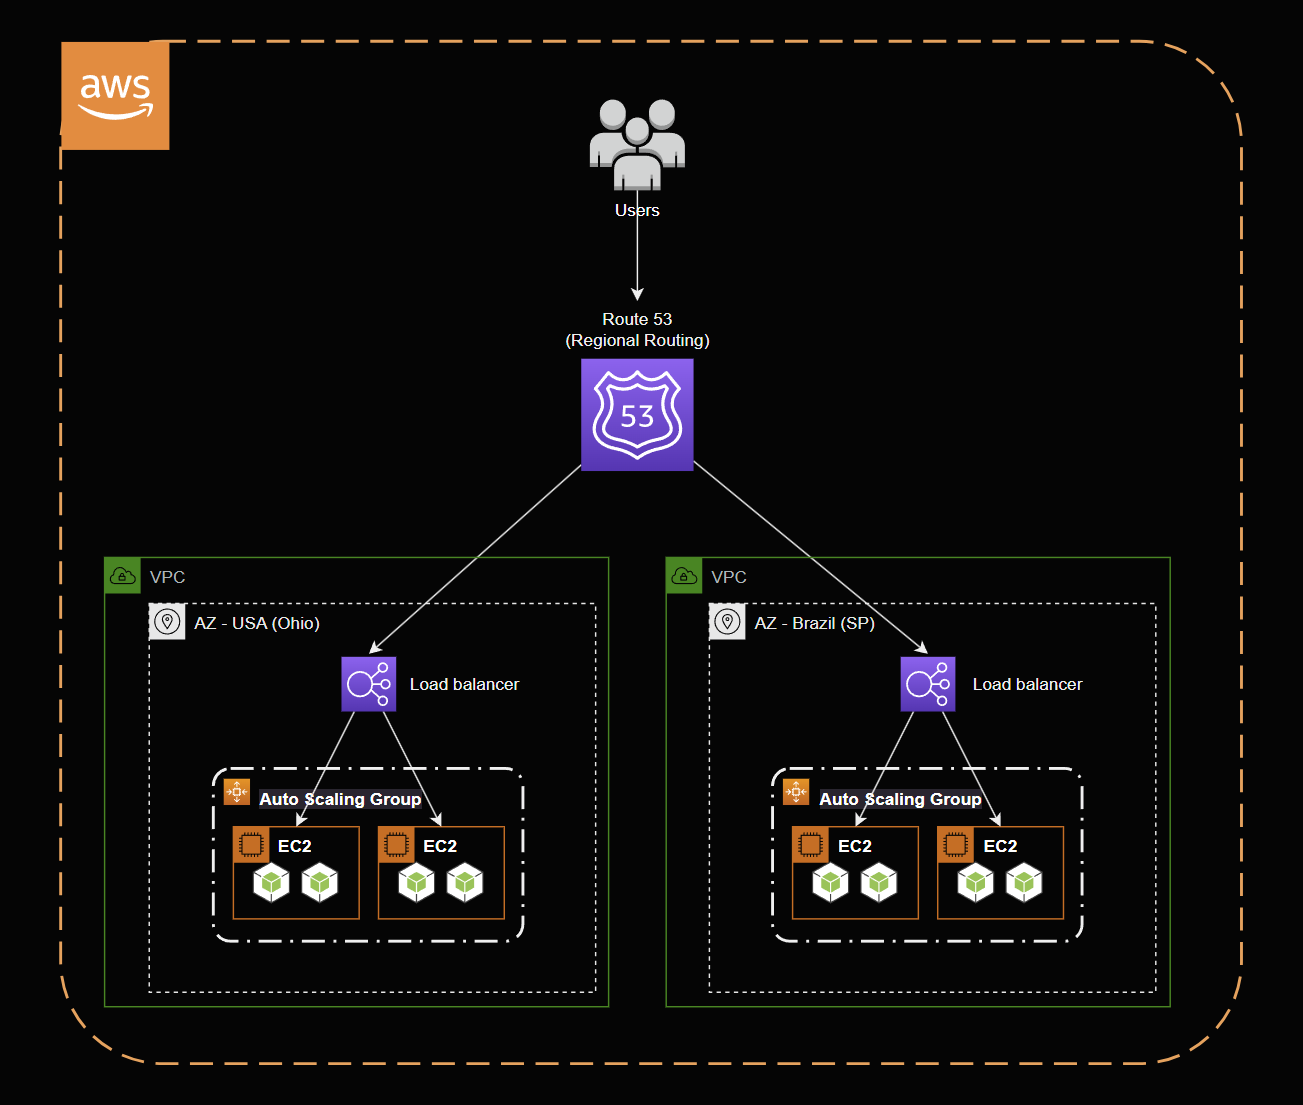
\includegraphics[width=\textwidth]{drawio/cloud-architecture.png}
    \caption{Visão Geral da Arquitetura em Nuvem}
    \label{fig:cloud-architecture}
\end{figure}

Essas práticas e tecnologias não apenas promovem a alta disponibilidade e desempenho da aplicação, mas também preparam o ambiente para escalar rapidamente em resposta às demandas crescentes, tudo sem intervenção manual, alinhando-se com as melhores práticas de DevOps e com as demandas de uma aplicação moderna.


\subsubsection{Planejamento de Infraestrutura}
% Revisado

O planejamento da infraestrutura da plataforma começou com a definição de requisitos e necessidades específicas da aplicação, que incluem:

\begin{itemize}
    \item \textbf{Baixa latência}: Para assegurar uma experiência de usuário fluida e responsiva em tempo real, a plataforma Codeboard precisa operar com baixa latência.
    \item \textbf{Alta disponibilidade}: Codeboard deve estar acessível 24/7, garantindo operação contínua, mesmo durante atualizações e manutenções.
    \item \textbf{Escalabilidade}: A plataforma deve suportar um grande número de usuários simultâneos, aumentando ou diminuindo seus recursos conforme a demanda.
    \item \textbf{Resiliência}: Codeboard precisa de mecanismos de recuperação automática frente a falhas de hardware ou software, sem impacto na experiência do usuário.
    \item \textbf{Custo-efetividade}: A infraestrutura deve ser otimizada para minimizar custos, evitando ociosidade de recursos.
    \item \textbf{Facilidade de gerenciamento}: a infraestrutura deve ser simples de gerenciar, utilizando práticas de DevOps, como \emph{Infra-as-Code} (IaC).
    \item \textbf{Segurança}: A plataforma deve ser protegida contra ameaças e ataques cibernéticos.
    \item \textbf{Monitoramento}: A plataforma deve contar com métricas e logs para acompanhar desempenho e integridade.
\end{itemize}

A hospedagem na Amazon Web Services (AWS) tornou-se uma escolha estratégica devido à sua ampla variedade de serviços, escalabilidade, confiabilidade e presença global de data centers. A infraestrutura global da AWS habilita a arquitetura \emph{Multi-Region Active-Active}, crucial para atender aos requisitos de desempenho e disponibilidade descritos.  Além disso, o \emph{free tier} da AWS foi um diferencial importante, possibilitando o desenvolvimento e os testes iniciais sem custos significativos.

Para atender a esses requisitos, foram escolhidos os seguintes serviços da AWS para compor a infraestrutura da plataforma Codeboard:

\begin{itemize}
    \item \textbf{Amazon Elastic Compute Cloud (EC2)}: Fornece instâncias virtuais escaláveis e seguras para execução da aplicação.
    \item \textbf{Amazon Elastic Load Balancing (ELB)}: Distribui o tráfego entre instâncias EC2, garantindo alta disponibilidade e escalabilidade.
    \item \textbf{AWS Auto Scaling}: Ajusta automaticamente a capacidade das instâncias EC2 conforme a demanda.
    % \item \textbf{Amazon DocumentDB}: serviço de banco de dados NoSQL que fornece instâncias gerenciadas de bancos de dados MongoDB.
    % \item \textbf{Amazon ElastiCache}: serviço de cache em memória que fornece instâncias gerenciadas de Redis.
    \item \textbf{Amazon Virtual Private Cloud (VPC)}: Cria uma rede virtual com sub-redes privadas, gateways de internet e regras de firewall.
    \item \textbf{Amazon Route 53}: Configura registros de DNS, oferece balanceamento de carga entre regiões geográficas e failover.
    \item \textbf{Amazon CloudWatch}: Proporciona métricas, logs e alarmes para monitorar a saúde e o desempenho da aplicação.
    \item \textbf{AWS Identity and Access Management (IAM)}: Gerencia o controle de acesso, permitindo a criação de usuários, grupos e políticas.
    \item \textbf{AWS Certificate Manager (ACM)}: Facilita a criação, renovação e implantação de certificados SSL/TLS para segurança de dados.
\end{itemize}

Essas escolhas de serviço atendem diretamente às necessidades de desempenho, segurança e custo, alinhando a infraestrutura às metas de alta disponibilidade e resiliência exigidas pela plataforma.


\subsubsection{Implementação de Infraestrutura como Código com Terraform}
% Revisado

Para assegurar um processo de implantação de infraestrutura que seja eficiente, escalável e replicável, a plataforma Codeboard utiliza o \emph{Terraform} como ferramenta de \emph{Infrastructure as Code} (IaC). Terraform permite definir a infraestrutura como código, o que possibilita o versionamento, automação e repetibilidade do processo de provisão da infraestrutura em nuvem.

Uma das principais vantagens do uso do Terraform é a capacidade de descrever toda a arquitetura em arquivos de configuração que podem ser facilmente armazenados, revisados e auditados. Ele utiliza sua própria linguagem, HCL (HashiCorp Configuration Language), que permite definir recursos da AWS, como instâncias EC2, balanceadores de carga, grupos de segurança e outros componentes necessários. O Terraform então interage diretamente com a API da AWS para provisionar e gerenciar esses recursos.

Além disso, o uso do Terraform garante que a infraestrutura seja declarativa e idempotente, o que significa que recursos existentes não são recriados desnecessariamente a cada execução. Isso resulta em um gerenciamento mais eficiente dos recursos e em um controle de mudanças mais preciso. Foram estabelecidos módulos Terraform para tratar de diferentes aspectos da infraestrutura, como rede, segurança e recursos de computação, permitindo que seja possível trabalhar isoladamente em partes distintas da arquitetura sem necessidade de intervenção manual entre essas partes.


\subsection{Infraestrutura de Computação}

Dada a adoção do modelo \emph{Multi-Region Active-Active}, a infraestrutura de computação da Codeboard foi arquitetada para operar de maneira distribuída através de diferentes regiões geográficas da AWS. Essa abordagem garante, além de uma resposta eficiente a eventuais falhas regionais, uma proximidade maior com os usuários, o que ajuda a reduzir a latência. A infraestrutura de computação integra múltiplos componentes, incluindo instâncias EC2, balanceamento de carga, escalabilidade automática, monitoramento, e diversos mecanismos para segurança e recuperação de falhas, criando um ambiente robusto que sustenta a operação contínua e eficiente da plataforma Codeboard.

\subsubsection{Servidor Virtual}
% Revisado

Para hospedar a aplicação da plataforma Codeboard, foram escolhidas instâncias EC2 do tipo \emph{t3.micro}, adequadas ao estudo de caso pelos seguintes motivos: 

\begin{itemize}
    \item \textbf{Custo}: As instâncias t3.micro fazem parte do \emph{free tier} da AWS, oferecendo 12 meses de uso gratuito, o que torna essa opção financeiramente viável para a fase inicial do projeto.
    \item \textbf{Desempenho Escalável}: Com capacidade de burst, essas instâncias podem fornecer recursos adicionais de CPU temporariamente, sem custos extras, atendendo a picos de demanda.
    \item \textbf{2 vCPUs}: As instâncias t3.micro possuem 2 vCPUs, que é o mínimo recomendado para a aplicação da plataforma Codeboard, que opera em um \emph{cluster} de processos, onde cada processo é uma aplicação Node.js que é responsável pelo backend.
    \item \textbf{1 GB de memória RAM}: A memória de 1 GB é adequada para a Codeboard, pois sua função de intermediação de mensagens em tempo real requer um baixo consumo de memória.
    \item \textbf{Armazenamento em disco SSD}: Embora a Codeboard não faça uso intensivo de disco, o armazenamento SSD nas instâncias t3.micro oferece maior velocidade e confiabilidade, beneficiando a estabilidade do sistema.
\end{itemize}

As instâncias EC2 foram configuradas com o sistema operacional \emph{Ubuntu 24.04 LTS}, o servidor web \emph{NGINX}, o gerenciador de processos \emph{PM2} e entre outras ferramentas. A escolha do Ubuntu 24.04 LTS deve-se à sua estabilidade e suporte de longo prazo para atualizações de segurança. O NGINX atua como um servidor web reverso, redirecionando o tráfego HTTPS para os processos Node.js que executam a Codeboard. Já o PM2 gerencia esses processos, mantendo-os ativos e reiniciando automaticamente em caso de falhas.

\subsection{Balanceamento de Carga, Escalabilidade e Recuperação de Falhas}
% Revisado

A arquitetura da plataforma Codeboard foi projetada com uma estratégia de balanceamento de carga, escalabilidade e recuperação de falhas que abrange múltiplos níveis de operação, assegurando alta disponibilidade, baixa latência e resiliência. Esta seção apresenta a abordagem utilizada para distribuir de forma eficiente o tráfego e garantir que a aplicação responda de maneira otimizada, mesmo em cenários de alta demanda ou falhas inesperadas.

Em primeiro lugar, o balanceamento de carga entre processos permite uma distribuição equitativa das requisições entre processos individuais da aplicação, garantindo o uso eficiente dos recursos da instância. Para lidar com o tráfego em servidores múltiplos, foi configurado um segundo nível de balanceamento de carga que distribui as requisições entre instâncias EC2 da AWS, de modo que a aplicação possa escalar horizontalmente conforme a demanda. Por fim, para maximizar a disponibilidade global e reduzir a latência para usuários em diferentes localidades, foi implementado um balanceamento de carga geográfico entre regiões da AWS, utilizando o Route 53 para redirecionar o tráfego para a região mais próxima do usuário.

Além disso, mecanismos de recuperação automática de falhas foram configurados em cada nível. Esses mecanismos monitoram continuamente a saúde dos processos e das instâncias, substituindo automaticamente recursos que falhem e garantindo a continuidade da aplicação. Essa estrutura multissetorial de balanceamento e recuperação permite que a plataforma Codeboard mantenha uma operação robusta e confiável, capaz de lidar com flutuações de carga e com interrupções inesperadas.

\subsubsection{Balanceamento de Carga entre Processos}
% Revisado

A aplicação Codeboard opera em um \emph{cluster} de processos, o que torna o balanceamento de carga essencial para distribuir o tráfego de entrada de maneira eficiente. Para isso, o PM2 foi configurado no modo cluster, permitindo a criação de múltiplos processos Node.js que compartilham o mesmo \emph{socket} de rede. Dessa forma, o NGINX redireciona o tráfego entre os processos por meio do módulo \emph{proxy\_pass}, que envia as requisições HTTP para o processo Node.js que executa a Codeboard.

O algoritimo de balanceamento de carga utilizado é o \emph{Round Robin}, que distribui o tráfego de entrada de forma alternada entre os processos do cluster, assegurando que cada processo receba uma quantidade igual de solicitações. A Figura \ref{fig:round-robin-load-balancing} ilustra o funcionamento do algoritmo Round Robin, enqunato a Figura \ref{fig:pm2-cluster-mode} mostra o modo cluster do PM2 em ação.

\begin{figure}[H]
    \centering
    \includegraphics[width=\textwidth]{diagrams/round-robin-load-balancing.png}
    \caption{Balanceamento de Carga com Round Robin}
    \label{fig:round-robin-load-balancing}
\end{figure} 

\begin{figure}[H]
    \centering
    \includegraphics[width=\textwidth]{diagrams/pm2-cluster-mode.png}
    \caption{Modo Cluster do PM2}
    \label{fig:pm2-cluster-mode}
\end{figure}

O balanceamento de carga entre processos otimiza o uso dos recursos de CPU e memória, distribuindo a carga de trabalho de maneira uniforme entre os vCPUs das instâncias EC2, garantindo um desempenho estável e eficiente.

\subsubsection{Recuperação Automática de Falhas em Processos}
% Revisado

O balanceamento de carga entre processos também contribui para a alta disponibilidade e confiabilidade da aplicação. Em caso de falha de um dos processos, o tráfego é automaticamente redirecionado para outros, evitando interrupções para os usuários.

Para reforçar a tolerância a falhas e garantir a alta disponibilidade, foram configurados no PM2 mecanismos de monitoramento e recuperação automática. Esse monitoramento verifica continuamente os processos Node.js e, ao detectar uma falha, reinicia o processo comprometido. A Figura\ref{fig:pm2-fault-tolerance} ilustra o funcionamento do monitoramento e recuperação de falhas pelo PM2, garantindo que a aplicação permaneça em funcionamento mesmo diante de falhas pontuais.


\begin{figure}[H]
    \centering
    \includegraphics[width=0.75\textwidth]{diagrams/pm2-fault-tolerance.png}
    \caption{Tolerância à Falhas com PM2}
    \label{fig:pm2-fault-tolerance}
\end{figure}


\subsubsection{Balanceamento de Carga entre os Servidores}
% Revisado

A infraestrutura de computação da plataforma Codeboard foi projetada para ser distribuída e redundante, assegurando que o tráfego seja balanceado entre várias instâncias EC2 e entre diferentes regiões geográficas. Para essa finalidade, utilizou-se o AWS Elastic Load Balancing (ELB), que distribui o tráfego de entrada de forma equilibrada entre as instâncias, garantindo alta disponibilidade e escalabilidade da aplicação.

Entre os tipos de ELB disponíveis, como o Application Load Balancer (ALB), Network Load Balancer (NLB) e Classic Load Balancer (CLB), escolheu-se o ALB. Esse balanceador de camada 7 permite o roteamento de tráfego com base em critérios específicos, como URL, cabeçalhos HTTP e métodos HTTP. O ALB foi configurado com um certificado SSL para assegurar a segurança do tráfego HTTPS entre clientes e servidores.

O algoritmo de balanceamento de carga adotado foi o \emph{Round Robin}, que distribui o tráfego de forma equitativa entre as instâncias EC2, garantindo uma divisão equilibrada de requisições.


% TODO: Voltar no capítulo 3 para explicar a importância do Health Check? Testar se a conexão com o banco de dados está funcionando, se a aplicação está respondendo, etc.

Para garantir que apenas instâncias saudáveis recebam tráfego, foram configurados \emph{Health Checks} para monitorar a saúde das instâncias EC2. Os Health Checks realizam verificações periódicas em uma rota específica da aplicação Codeboard, permitindo que o ELB detecte se cada instância está respondendo corretamente. Se uma instância não responder adequadamente ao Health Check, o ELB a marca como indisponível e redireciona o tráfego para outras instâncias saudáveis.

Configurou-se o Health Check com um intervalo de 30 segundos e um tempo limite de 5 segundos, o que significa que o ELB realiza uma verificação a cada 30 segundos e aguarda uma resposta dentro de 5 segundos. Após duas falhas consecutivas, a instância é marcada como indisponível e o tráfego é redirecionado para outras instâncias saudáveis. A Figura \ref{fig:elb-health-check} ilustra o funcionamento do Health Check do ELB.

\begin{figure}[H]
    \centering
    \includegraphics[width=0.75\textwidth]{diagrams/elb-health-check.png}
    \caption{Health Check do ELB}
    \label{fig:elb-health-check}
\end{figure}


\subsubsection{Escalabilidade Horizontal com Auto Scaling}
% Revisado

Para garantir a alta disponibilidade da plataforma Codeboard, a infraestrutura foi projetada para escalar horizontalmente, permitindo que a aplicação aumente ou reduza seus recursos de acordo com a demanda, sem necessidade de intervenção manual. Essa escalabilidade automática foi implementada com o AWS Auto Scaling, que ajusta a quantidade de instâncias EC2 com base na utilização de recursos.

O Auto Scaling utiliza um Auto Scaling Group (ASG) para monitorar a utilização de CPU nas instâncias EC2 e ajustar a quantidade de instâncias conforme uma política de escalabilidade. Definiram-se gatilhos específicos: quando a utilização de CPU ultrapassa um limite predefinido, uma nova instância é adicionada ao grupo, distribuindo melhor a carga. Inversamente, se a utilização de CPU cair abaixo de um limite, o ASG reduz o número de instâncias, otimizando custos. Foi configurado um número mínimo e máximo de instâncias, garantindo um custo controlado e uma capacidade mínima sempre disponível. A Figura \ref{fig:auto-scaling-horizontal-scalability} ilustra essa escalabilidade horizontal com o Auto Scaling.

\begin{figure}[H]
    \centering
    \includegraphics[width=\textwidth]{diagrams/auto-scaling-horizontal-scalability.png}
    \caption{Escalabilidade Horizontal com Auto Scaling Group}
    \label{fig:auto-scaling-horizontal-scalability}
\end{figure}

Os limites de gatilhos de escalabilidade foram definidos com base em testes e monitoramento da aplicação, estabelecendo 70\% de uso de CPU para adicionar uma nova instância e 30\% para removê-la. Os valores de instâncias mínima e máxima foram configurados entre 1 e 5, podendo ser ajustáveis conforme previsões de tráfego, sazonalidade e eventos especiais.

\subsubsection{Recuperação Automática de Falhas em Servidores}
% Revisado

O Auto Scaling do AWS também possui um mecanismo de recuperação automática de falhas, que monitora continuamente a saúde das instâncias EC2. Quando uma instância é marcada como indisponível pelo ELB (por falhar em um Health Check), o Auto Scaling substitui automaticamente a instância defeituosa por uma nova, garantindo que a aplicação da plataforma Codeboard permaneça sempre disponível e resiliente a falhas. Essa combinação de Auto Scaling, ELB e PM2 resulta em uma arquitetura altamente disponível, escalável e confiável. A Figura \ref{fig:auto-scaling-fault-tolerance} ilustra o funcionamento da recuperação automática de falhas com o Auto Scaling.

\begin{figure}[H]
    \centering
    \includegraphics[width=\textwidth]{diagrams/auto-scaling-fault-tolerance.png}
    \caption{Recuperação Automática de Falhas com Auto Scaling}
    \label{fig:auto-scaling-fault-tolerance}
\end{figure}

Durante a inicialização de uma nova instância, o Auto Scaling aplica um \emph{warmup time} de 180 segundos, período necessário para que a instância esteja completamente operacional. Nesse tempo, são realizadas tarefas como configuração da instância, inicialização da aplicação e estabelecimento de conexões com o banco de dados. Durante o warmup time, a instância permanece indisponível para o ELB, e o tráfego é direcionado para outras instâncias saudáveis. Após o término do warmup, a instância é marcada como disponível e começa a receber tráfego. Esse warmup time ajuda a evitar interrupções na aplicação, garantindo que apenas instâncias totalmente preparadas participem da distribuição de carga.


\subsubsection{Balanceamento de Carga entre Regiões Geográficas}
% Revisado

A infraestrutura da plataforma Codeboard foi projetada para operar em várias regiões geográficas da AWS, permitindo distribuição do tráfego de usuários entre essas regiões para assegurar alta disponibilidade e baixa latência. Essa configuração de várias regiões não só oferece resiliência em caso de falhas regionais (devido a desastres naturais, falhas de hardware, ou manutenção programada), mas também aproxima a aplicação dos usuários, o que reduz a latência e aprimora a experiência de uso.

Para essa distribuição de tráfego entre regiões, foi configurado o Amazon Route 53, o serviço de DNS da AWS que também oferece balanceamento de carga e failover. Um registro de DNS foi criado para a aplicação da plataforma Codeboard no Route 53, o qual direciona o tráfego para o ELB de cada região geográfica. Devido à natureza de comunicação em tempo real da plataforma, o Route 53 foi configurado com balanceamento de carga baseado em latência, de forma que redireciona o tráfego para a região geográfica mais próxima do usuário, garantindo uma experiência rápida e eficiente. A Figura \ref{fig:route-53-geographic-load-balancing} demonstra o funcionamento do balanceamento de carga baseado em latência do Route 53.

\begin{figure}[H]
    \centering
    \includegraphics[width=\textwidth]{diagrams/route-53-geographic-load-balancing.png}
    \caption{Balanceamento de Carga Baseado em Latência com Route 53}
    \label{fig:route-53-geographic-load-balancing}
\end{figure}

\subsection{Segurança da Infraestrutura}
% Revisado

A segurança da infraestrutura é um aspecto essencial para garantir a proteção dos dados e a continuidade das operações da plataforma Codeboard. Nesta seção, são discutidas as medidas de segurança implementadas para prevenir acesso não autorizado, proteger o tráfego de dados e garantir a confiabilidade da infraestrutura. Essas práticas abrangem desde o controle de acesso aos recursos de computação até a aplicação de criptografia de dados, assegurando a integridade e a privacidade das informações dos usuários. 

\subsubsection{Controle de Acesso}
% Revisado

Para proteger a infraestrutura computacional da plataforma Codeboard, várias políticas de segurança foram implementadas, incluindo:

\begin{itemize}
    \item \textbf{AWS Identity and Access Management (IAM)}: políticas e papéis no IAM foram criados para controlar o acesso aos recursos da AWS, aplicando o princípio do menor privilégio. As instâncias EC2, por exemplo, possuem permissões restritas, limitadas apenas às ações necessárias para o funcionamento da aplicação.
    \item \textbf{Firewall}: regras de firewall foram configuradas no \emph{Security Group} da VPC para restringir o tráfego de entrada e saída das instâncias EC2. Somente as portas essenciais para a aplicação estão abertas: a porta 80 (HTTP) é acessível apenas pelo ELB, enquanto a porta 22 (SSH) está disponível exclusivamente para IPs autorizados. Todas as demais portas de entrada são bloqueadas.
    \item \textbf{Chaves SSH}: chaves SSH foram geradas para garantir a autenticação segura de usuários no acesso remoto às instâncias EC2.
\end{itemize}

Além disso, as instâncias EC2 não são acessadas diretamente; o tráfego de entrada passa pelo ELB, que distribui as conexões de forma uniforme. O ELB está configurado com um certificado SSL para garantir a criptografia do tráfego entre cliente e servidor, protegendo os dados em trânsito. Seu Security Group permite apenas o tráfego de entrada na porta 443 (HTTPS).

\subsubsection{Criptografia de Dados em Trânsito}
% Revisado

A criptografia de dados em trânsito é uma técnica que protege as informações enquanto são transferidas entre diferentes pontos de uma rede, como entre o navegador de um usuário e um servidor. Ao criptografar esses dados, evita-se que terceiros consigam interceptá-los e acessá-los sem autorização, garantindo que apenas o remetente e o destinatário possam interpretá-los. Essa medida é fundamental para proteger a privacidade dos usuários e a integridade das informações, especialmente em plataformas que processam dados sensíveis, evitando problemas como roubo de informações e ataques de espionagem.

Para assegurar a segurança dos dados em trânsito, um certificado SSL foi configurado no ELB para criptografar o tráfego entre o cliente e o servidor. Esse certificado, emitido pelo AWS Certificate Manager (ACM), é gratuito e gerenciado, sendo adequado para serviços da AWS. A configuração inclui um domínio personalizado da plataforma Codeboard, disponível em https://codeboard.pitrol.dev/, o que garante a autenticidade e a integridade das conexões HTTPS. Com isso, a criptografia dos dados em trânsito protege contra interceptações e garante a privacidade e a segurança dos usuários.

% TODO?: \subsubsection{Rotatividade de Chaves e Segredos}

\subsection{Banco de Dados MongoDB}
% Revisado

O banco de dados escolhido para a plataforma Codeboard foi o MongoDB, uma solução NoSQL amplamente utilizada por sua flexibilidade, escalabilidade e alto desempenho em aplicações modernas. Diversas abordagens poderiam ser adotadas para hospedar o MongoDB, incluindo instalações locais, máquinas virtuais, contêineres Docker e serviços gerenciados na nuvem. No caso da Codeboard, optou-se pelo \emph{MongoDB Atlas}, um serviço gerenciado pela própria MongoDB que opera sobre infraestruturas robustas como a AWS, Google Cloud Platform e Microsoft Azure.

Essa escolha trouxe diversas vantagens, incluindo alta disponibilidade, escalabilidade e segurança integradas. O MongoDB Atlas proporciona funcionalidades como backups automáticos, monitoramento em tempo real, escalabilidade ajustável e criptografia de dados em trânsito e em repouso, além de integração com outros serviços da AWS. Para atender às necessidades iniciais da aplicação, foi selecionada a instância \emph{M10}, que oferece 2 GB de armazenamento e 0,5 GB de RAM, com suporte a escalabilidade para acomodar futuras demandas.

A adoção do MongoDB Atlas permite que a equipe foque no desenvolvimento da aplicação, enquanto a gestão do banco de dados é simplificada por meio de recursos automatizados, garantindo a robustez e a eficiência no gerenciamento dos dados da plataforma.


\subsubsection{Escalabilidade Vertical Automática}
% Revisado

O banco de dados MongoDB da plataforma Codeboard foi configurado para escalar verticalmente de maneira automática, garantindo que possa atender ao crescimento das demandas de forma eficiente. A escalabilidade vertical consiste em aumentar os recursos de uma única instância, como CPU, memória e armazenamento, sem a necessidade de configurar múltiplas réplicas ou lidar com a complexidade da escalabilidade horizontal.

A escolha pela escalabilidade vertical, em vez da horizontal, foi fundamentada por duas razões principais:
\begin{enumerate}
    \item \textbf{Custo e Complexidade}: A escalabilidade horizontal envolve a distribuição de dados e cargas de trabalho entre múltiplas instâncias, o que requer configurações avançadas e ferramentas específicas, como sharding. Para um banco de dados com baixa utilização de recursos, a escalabilidade horizontal representaria um custo desnecessário e maior complexidade operacional.
    \item \textbf{Adequação ao Escopo Atual}: O uso inicial da instância M10 do MongoDB Atlas, com 2 GB de armazenamento e 0,5 GB de RAM, provou ser suficiente para as necessidades da aplicação. No entanto, a escalabilidade vertical automática garante que, conforme a demanda cresça, a infraestrutura acompanhe esse crescimento sem interrupções.
\end{enumerate}

O MongoDB Atlas permite configurar a escalabilidade vertical de forma automática, ajustando a capacidade da instância com base na utilização de recursos. Os gatilhos predefinidos monitoram métricas de desempenho, como:
\begin{itemize}
    \item \textbf{CPU}: Se a utilização ultrapassar um limite definido (e.g., 80\%) por um período contínuo, a capacidade da instância é aumentada automaticamente.
    \item \textbf{Memória}: Um uso persistente acima de uma faixa segura dispara o aumento de recursos.
    \item \textbf{Armazenamento}: Quando o espaço disponível atinge um limite crítico (e.g., 85\%), a capacidade de armazenamento é ampliada.
\end{itemize}


Da mesma forma, a escalabilidade vertical também reduz a capacidade da instância quando os recursos são subutilizados, ajudando a otimizar custos operacionais sem sacrificar o desempenho. A Figura \ref{fig:mongodb-atlas-vertical-scalability} ilustra o funcionamento da escalabilidade vertical automática configurada no MongoDB Atlas.

\begin{figure}[H]
    \centering
    \includegraphics[width=\textwidth]{diagrams/mongodb-atlas-vertical-scalability.png}
    \caption{Escalabilidade Vertical Automática no MongoDB Atlas}
    \label{fig:mongodb-atlas-vertical-scalability}
\end{figure} 

Os benefícios da escalabilidade vertical automática no MongoDB Atlas são diversos e contribuem significativamente para a eficiência operacional da plataforma Codeboard, diminuindo a complexidade, reduzindo custos e automatizando o gerenciamento de recursos do banco de dados. Essa abordagem garante que o banco esteja sempre preparado para atender às demandas crescentes da aplicação, sem a necessidade de interrupções ou intervenções manuais.


\subsubsection{Backup, Controle de Acesso e Segurança de Dados}
% Revisado

Para atender aos requisitos de segurança e confiabilidade da plataforma Codeboard, foi implementada uma estratégia robusta que abrange tanto o gerenciamento de backups quanto o controle de acesso ao banco de dados e a proteção dos dados em trânsito e em repouso.

Os backups automáticos realizados pelo MongoDB Atlas garantem a preservação e recuperação de dados em caso de falhas ou perdas acidentais, com uma política de retenção que permite a restauração para pontos no tempo ao longo de 14 dias. Adicionalmente, backups sob demanda oferecem flexibilidade para proteger os dados em momentos críticos, como antes de atualizações ou mudanças significativas.

No que diz respeito à segurança, políticas rigorosas de controle de acesso foram implementadas para restringir conexões não autorizadas. Isso inclui o uso de \emph{Whitelists} de IPs e autenticação com credenciais específicas para diferentes níveis de permissão. Além disso, a criptografia de dados, tanto em trânsito quanto em repouso, protege contra interceptações e acessos indevidos, utilizando tecnologias SSL e armazenamento seguro no MongoDB Atlas.

Essas medidas asseguram que os dados da plataforma permaneçam seguros, disponíveis e protegidos contra uma ampla gama de riscos e ameaças.

\subsection{Banco de dados Redis}
% Revisado

O Redis desempenha um papel crucial na infraestrutura da plataforma Codeboard, servindo como um banco de dados chave-valor em memória de alta performance. Sua velocidade, simplicidade e capacidade de escalabilidade o tornam ideal para atender às necessidades de aplicações que exigem processamento rápido de dados em tempo real, como é o caso da Codeboard. Nesta seção, serão explorados os detalhes de sua configuração, os benefícios de utilizar uma solução gerenciada e as práticas implementadas para garantir a segurança, disponibilidade e desempenho do banco de dados.

\subsubsection{Provedor de Banco de Dados}
% Revisado

O banco de dados Redis da plataforma Codeboard está hospedado no \emph{Redis Cloud}, uma solução gerenciada pela própria Redis. Essa escolha foi motivada pela robustez e confiabilidade do serviço, que elimina a necessidade de gerenciamento manual da infraestrutura de banco de dados, além de oferecer recursos avançados como monitoramento, backup e suporte técnico especializado.

O Redis Cloud proporciona uma infraestrutura otimizada para alta disponibilidade e desempenho, com suporte a escalabilidade automática para lidar com variações de carga. Além disso, o uso de uma solução gerenciada permite que a equipe foque no desenvolvimento e na operação da aplicação, ao invés de dedicar tempo e recursos ao gerenciamento do banco de dados.

\subsubsection{Sharding e Replicação}
% Revisado

Para garantir alta disponibilidade e baixa latência, o Redis foi configurado com sharding e replicação. A abordagem de escalabilidade horizontal, baseada no sharding, distribui os dados entre múltiplas réplicas em diferentes nós, permitindo que o banco de dados suporte um grande volume de transações simultâneas sem comprometer o desempenho.

O sharding foi configurado de forma automática pelo Redis Cloud, que gerencia a alocação de dados e o balanceamento de carga entre shards. Já a replicação assegura a resiliência do sistema, criando réplicas secundárias de cada shard. Em caso de falha de um nó, o Redis Cloud promove automaticamente uma réplica para substituí-lo, garantindo continuidade no serviço.

\subsubsection{Controle de Acesso e Segurança}
% Revisado

A segurança do banco de dados Redis foi configurada com foco em prevenir acessos não autorizados e proteger os dados transmitidos. As políticas de controle de acesso incluem autenticação por senha e restrições baseadas em IP, permitindo conexões apenas de hosts autorizados. Essa abordagem reduz significativamente o risco de acessos externos indevidos.

Para garantir a proteção dos dados em trânsito, o tráfego entre os clientes e o Redis é criptografado utilizando TLS, prevenindo interceptações e acessos maliciosos.

Dado o papel do Redis na plataforma Codeboard, que é utilizado principalmente para dados temporários, não foram configurados backups automáticos. Os dados críticos da aplicação são armazenados no MongoDB, que conta com backups automáticos e políticas de retenção robustas. Essa estratégia assegura que, mesmo em caso de perda de dados no Redis, eles possam ser facilmente regenerados sem impacto significativo na operação.


\subsection{Distribuição de Conteúdo (CDN)}
% Revisado

Uma \emph{Content Delivery Network} (CDN) é uma rede de servidores distribuídos geograficamente que trabalham em conjunto para entregar conteúdos da web com rapidez e eficiência. Ao armazenar cópias dos arquivos em locais próximos aos usuários finais, uma CDN reduz o tempo de carregamento, diminui a carga no servidor de origem e melhora a experiência do usuário.

\subsubsection{Plataforma de CDN}
% Revisado

A utilização de uma CDN desempenha um papel essencial na entrega rápida e eficiente do front-end da plataforma Codeboard. A infraestrutura foi implementada utilizando a plataforma \emph{Vercel}, que combina os benefícios de uma CDN global com recursos de plataforma como serviço (PaaS), otimizando a experiência dos usuários finais.

O uso da CDN integrada ao Vercel traz diversos benefícios, incluindo:

\begin{itemize}
    \item Redução de latência: Ao distribuir o conteúdo para servidores localizados próximos aos usuários, o tempo de resposta é minimizado.
    \item Alta disponibilidade: A CDN utiliza redundância para garantir que os conteúdos estejam sempre acessíveis, mesmo em caso de falhas em servidores específicos.
    \item Escalabilidade automática: A infraestrutura da CDN lida automaticamente com picos de tráfego, assegurando desempenho consistente.
    \item Segurança aprimorada: Recursos como mitigação de DDoS e controle de acesso a nível de borda ajudam a proteger a plataforma contra ataques.
\end{itemize}

\subsubsection{Configuração da CDN}
% Revisado

No contexto da Codeboard, a configuração da CDN foi simplificada pela utilização do Vercel. A plataforma automaticamente gerencia o cache de conteúdo estático e implementa o cache dinâmico conforme necessário, baseado nos cabeçalhos de resposta configurados na aplicação. Regras de invalidade de cache são aplicadas automaticamente durante os deploys, garantindo que os usuários sempre acessem a versão mais recente da aplicação.

Além disso, a CDN do Vercel está totalmente integrada com o sistema de build e deploy contínuos, sincronizando alterações no front-end com a rede de distribuição em tempo real. Essa abordagem garante alta performance e agilidade no lançamento de novas funcionalidades.


\subsection{Monitoramento}
% Revisado

% Por que monitoramento é importante? R: Garantir a disponibilidade, desempenho e segurança da aplicação, atuando proativamente para evitar falhas e interrupções.

O monitoramento é um elemento crítico para garantir a disponibilidade, o desempenho e a segurança da aplicação. Por meio do acompanhamento contínuo de métricas e logs, é possível identificar e mitigar problemas proativamente, antes que causem interrupções ou degradação no serviço. Esta seção detalha como o monitoramento é implementado na plataforma Codeboard, abrangendo tanto a aplicação quanto os recursos de infraestrutura em nuvem.

\subsubsection{Monitoramento da Aplicação}
% Revisado

% Como o monitoramento da aplicação é feito? R: CloudWatch
% Quais métricas são monitoradas? R: Requisições, logs de erros, etc.

O monitoramento da aplicação é realizado utilizando o \emph{Amazon CloudWatch}, um serviço nativo da AWS que permite coletar, analisar e agir com base em dados e logs de desempenho. As métricas monitoradas incluem:

\begin{itemize}
    \item \textbf{Requisições}: Número de requisições recebidas, permitindo analisar padrões de tráfego e identificar possíveis gargalos.
    \item \textbf{Logs de erros}: Registro de falhas e exceções capturados em tempo real, possibilitando a identificação de problemas no código ou na infraestrutura.
    \item \textbf{Latência}: Tempo médio de resposta das requisições, monitorando a eficiência da aplicação e identificando possíveis pontos de melhoria.
\end{itemize}

Os dados coletados são apresentados em dashboards personalizados, oferecendo uma visão consolidada da saúde da aplicação e facilitando a identificação de padrões anormais.


\subsubsection{Monitoramento de Recursos da Nuvem}
% Revisado

% Como o monitoramento de recursos da nuvem é feito? R: CloudWatch
% Quais métricas são monitoradas? R: CPU, memória, etc.

Além da aplicação, os recursos da infraestrutura de computação em nuvem também são monitorados por meio do Amazon CloudWatch. Essa abordagem assegura que os componentes subjacentes, como os servidores, operem dentro dos parâmetros esperados.

As principais métricas monitoradas incluem:

\begin{itemize}
    \item \textbf{Uso de CPU}: Percentual de utilização do processador, indicando se os recursos estão sendo subutilizados ou sobrecarregados.
    \item \textbf{Uso de memória}: Quantidade de memória consumida, essencial para evitar problemas de desempenho devido à falta de recursos.
    \item \textbf{Tamanho de disco}: Utilização de armazenamento, permitindo antecipar a necessidade de expansão.
\end{itemize}

O monitoramento desses recursos é fundamental para identificar gargalos de desempenho e escalonar a infraestrutura de maneira eficiente.

\subsubsection{Alertas e Notificações}
% Revisado

O sistema de monitoramento da plataforma Codeboard conta com uma estratégia robusta de alertas para garantir respostas rápidas a possíveis incidentes. Os alertas são configurados no Amazon CloudWatch, permitindo a detecção e notificação de anomalias em tempo real.

As principais características do sistema de alertas incluem critérios personalizáveis, permitindo a configuração de limites para métricas específicas, como latência acima de 500ms, uso de CPU superior a 80\% ou erros 5xx que excedam um determinado volume. Além disso, há integração com ferramentas de comunicação, com notificações automáticas enviadas para canais como Slack e e-mail, garantindo que os responsáveis sejam informados imediatamente.

Com essa abordagem, o sistema de alertas fortalece a capacidade da plataforma de reagir rapidamente a eventos adversos, reduzindo o impacto nos usuários e assegurando a continuidade do serviço.

\section{Testes e Resultados}
To do

\newpage
\nocite{*}
\bibliographystyle{plain}
\bibliography{references.bib}

\end{document}